% June 2015 (TOC contents linked in blue in pdf file)
%This template was prepared by Dorothea F. Brosius of the 
%Institute for Electronics and Applied Physics, University of Maryland, College Park, MD
%The template was last updated in June 2015
%Thesis Main Page used with thesis.sty based on the
%University of Maryland Electronic Thesis and Dissertation (ETD) Style Guide (2014)

%The YourInformation file was created by Freja Nordsiek, 2014.
%Code for linking the TOC titles to the text in the pdf file was created by Freja Nordsiek, 2014.


% Select the version that fits how you are making this LaTeX document (its driver).
% The first two are the most likely ones to be needed.
%
% \newcommand{\mydriver}{pdftex} %Making a PDF directly using pdflatex.
%\newcommand{\mydriver}{dvipdfmx} %Making a DVI and converting that to PDF using dvipdfmx.
% \newcommand{\mydriver}{dvipdfm} %Making a DVI and converting that to PDF using dvipdfm.
 \newcommand{\mydriver}{dvips} %Making a DVI and converting that to PS using dvips (may later be converted to PDF).  (Used with my pc)
% \newcommand{\mydriver}{dvipsone} %Making a DVI and converting that to PS using dvipsone (may later be converted to PDF).
% \newcommand{\mydriver}{ps2pdf} %Same as the one for dvips except it is compatible with Ghostscript's PDF writer.


\documentclass[12pt,\mydriver]{thesis}  %12pt is larger than 11pt

\usepackage{titlesec}
   \titleformat{\chapter}
      {\normalfont\large}{Chapter \thechapter:}{1em}{}

\usepackage{graphicx}
\usepackage{cite}
\usepackage{lscape}
\usepackage{indentfirst}
\usepackage{latexsym}
\usepackage{multirow}
\usepackage{tabls}
\usepackage{wrapfig}
\usepackage{slashbox}
\usepackage{longtable}
\usepackage{supertabular}
\usepackage{subeqn}
\usepackage{subfigure}
\usepackage[dvips, bookmarks, colorlinks=true, plainpages=false, citecolor=blue, urlcolor=blue, filecolor=blue, linkcolor=blue]{hyperref} 
	%Works with PcTex.  You may have to choose one of the drivers above if dvips does not work.

\newcommand{\tbsp}{\rule{0pt}{18pt}} %used to get a vertical distance after \hline
\renewcommand{\baselinestretch}{2}
\setlength{\textwidth}{5.9in}
\setlength{\textheight}{9in}
\setlength{\topmargin}{-.50in}
%\setlength{\topmargin}{0in}    %use this setting if the printer makes the the top margin 1/2 inch instead of 1 inch
\setlength{\oddsidemargin}{.55in}
\setlength{\parindent}{.4in}
\pagestyle{empty}

\begin{document}

% !TEX root = mainthesis.tex
%Abstract Page 

\hbox{\ }

\renewcommand{\baselinestretch}{1}
\small \normalsize

\begin{center}
\large{{ABSTRACT}} 

\vspace{3em} 

\end{center}
\hspace{-.15in}
\begin{tabular}{ll}
Title of dissertation:   
&				      {\large  EXPERIMENTS WITH} \\
&				      {\large  STUFF IN THE LAB} \\
\ \\
&                     {\large  Ana Valdés-Curiel,} \\
&					  {\large  Doctor of Philosophy, 2019} \\
\ \\
Dissertation directed by: & {\large  Professor Ian Spielman} \\
&  							{\small	 Joint Quantum Institute,} \\
&  							{\small	 National Institute of Standards and Technology and} \\
&  							{\small	 University of Maryland College Park} \\
\end{tabular}

\vspace{3em}

\renewcommand{\baselinestretch}{2}
\large \normalsize

This thesis describes some of the work I did. It doesn't include work I didn't do. It mentions some of the work I had others do for me and finally some of the work others had me do for them.


 %(must be first, required, non-numbered)
%Titlepage

\thispagestyle{empty}
\hbox{\ }
\vspace{1in}
\renewcommand{\baselinestretch}{1}
\small\normalsize
\begin{center}

\large{{EGINEERING TOPOLOGICAL MATTER WITH ULTA-COLD ATOMS}}
\ \\
\ \\
\large{by} \\
\ \\
\large{Ana Vald\'es Curiel}%Your full name as it appears in University records.
\ \\
\ \\
\ \\
\ \\
\normalsize
Dissertation submitted to the Faculty of the Graduate School of the \\
University of Maryland, College Park in partial fulfillment \\
of the requirements for the degree of \\
Doctor of Philosophy \\
2019
\end{center}

\vspace{7.5em}

\noindent Advisory Committee: \\
Dr. Ian Spielman, Advisor \\
Rattata, cites Meowth \\
Meowth, cites Pikachu \\
Squirtle, cites self \\
Pikachu, cites Meowth
 %(must follow Abstract, required, non-numbered)
%Copyright

\thispagestyle{empty}
\hbox{\ }

\vfill
\renewcommand{\baselinestretch}{1}
\small\normalsize

\vspace{-.65in}

\begin{center}
\large{\copyright \hbox{ }Copyright by\\
Francisco Salces-Carcoba  %Type your name as it appears in University records
\\
2018}
\end{center}

\vfill
 %(highly recommended, non-numbered)

%Pages from this point start at lower-case Roman number ii)
\pagestyle{plain}
\pagenumbering{roman}
\setcounter{page}{2}

%Preface

\renewcommand{\baselinestretch}{2}
\small\normalsize
\hbox{\ }
 
\vspace{-.65in}

\begin{center}
\large{Preface} 
\end{center} 

A few weeks after I had started writing this thesis Ian came to me and asked if I had learned all the physics I wish I had known while I was doing my PhD. I felt a bit puzzled. I had been operating the lab, analyzing data and writing papers for a while, of course I already knew the physics relevant to my research! It finally hit me when I was writing the introductory chapters how many subtleties I had missed and how much I still didn't know. As experimental physicists being in the lab can give us some physical intuition and a sense of understanding but sometimes that is not enough. This was a very striking and unexpected side effect of the thesis and I invite experimentalists reading this to challenge their lab intuition. 

In the end, I actually found it very enjoyable to look back at the history of our field and to put my research into a bigger context. I never thought the words thesis and  enjoyable could go well together! My advice for a graduate student starting to write a thesis is try to enjoy the ride, it will definitely be stressful and overwhelming but try to make the best of it. 

Finally, I would like to mention that I wrote a lot of this thesis with new students in the lab in mind hoping it will be a useful reference in their research.  %(if present, start at lower-case Roman number ii)
%Foreword

\renewcommand{\baselinestretch}{2}
\small\normalsize
\hbox{\ }
 
\vspace{-.65in}

\begin{center}
\large{Foreword} 
\end{center} 

If needed.
 %(if present, lower-case Roman)
%Dedication

\renewcommand{\baselinestretch}{2}
\small\normalsize
\hbox{\ }
 
\vspace{-.65in}

\begin{center}
\large{Dedication}
\end{center} 

If needed.
 %(if present, lower-case Roman)
%Acknowledgments

\renewcommand{\baselinestretch}{2}
\small\normalsize
\hbox{\ }
 
\vspace{-.65in}

\begin{center}
\large{Acknowledgments} 
\end{center} 

\vspace{1ex}

I owe my gratitude to all the people who have made this thesis possible and because of whom my graduate experience has been one that I will cherish forever.

First and foremost I'd like to thank my advisor, Professor Rajarshi Roy for giving me an invaluable opportunity to work on challenging and extremely interesting projects over the past four years. He has always made himself available for help and advice and there has never been an occasion when I've knocked on his door and he hasn't given me time. It has been a pleasure to work with and learn from such an extraordinary individual.

I would also like to thank my co-advisor, Dr. Parvez Guzdar. Without his extraordinary theoretical ideas and computational expertise, this thesis would have been a distant dream. Thanks are due to Professor Robert Gammon, Professor Edward Ott and Professor Thomas Antonsen for agreeing to serve on my thesis committee and for sparing their invaluable time reviewing the manuscript.

My colleagues at the nonlinear optics laboratory have enriched my graduate life in many ways and deserve a special mention. David DeShazer helped me start-off by rewriting the basic simulation code in a user-friendly format. Christian Silva provided help by setting up the GRENOUILLE apparatus and performing some of the simulations. My interaction with  Rohit Tripathi, Ryan McAllister, Vasily Dronov, Min-Young Kim, Elizabeth Rogers, William Ray, Jordi Garcia Ojalvo, Riccardo Meucci, Atsushi Uchida, and Fabian Rogister has been very fruitful. I'd also like to thank Wing-Shun Lam and Benjamin Zeff for providing the LaTex style files for writing this thesis.

I would also like to acknowledge help and support from some of the staff members. Donald Martin's technical help is highly appreciated, as is the computer hardware support from Edward Condon, LaTex and software help from Dorothea Brosius and purchasing help from Nancy Boone.

I owe my deepest thanks to my family - my mother and father who have always stood by me and guided me through my career, and have pulled me through against impossible odds at times. Words cannot express the gratitude I owe them. I would also like to thank Dr. Mohan Advani, Dr. Vasudeo Paralikar and Dr. Vinod Chaugule who are like family members to me.

My housemates at my place of residence have been a crucial factor in my finishing smoothly. I'd like to express my gratitude to Sivasankar Pandeti, Jayakumar Patil, Amit Trehan and Punyaslok Purakayastha for their friendship and support.

I would like to acknowledge financial support from the Office of Naval Research (ONR), Physics, for all the projects discussed herein.

It is impossible to remember all, and I apologize to those I've inadvertently left out.

Lastly, thank you all and thank God!
 %(if present, lower-case Roman)

\renewcommand{\baselinestretch}{1}
\small\normalsize
\tableofcontents %(required, lower-case Roman)
\newpage
%\listoftables %(if present, lower-case Roman)
%\newpage
\listoffigures %(if present, lower-case Roman)
\newpage
% LIST OF ABBREVIATIONS
\addcontentsline{toc}{chapter}{List of Abbreviations}
%List of Abbreviations

\renewcommand{\baselinestretch}{1}
\small\normalsize
\hbox{\ }

\vspace{-3em}


\begin{center}
\large{List of Abbreviations}
\end{center} 

\vspace{3pt}

\begin{tabular}{ll}
Abbreviation & Full meaning \\
BEC & Bose-Einstein condensate \\
SOC & spin-orbit coupling \\
RbLi & Rubidium-Lithium \\
DD & dynamical decoupling \\  
CDD & continuous dynamical decoupling \\
TOF & time of flight \\
OD & optical depth \\
TF & Thomas-Fermi \\
MOT & magneto optical trap \\
RF & radio frequency \\
ARP & adiabatic rapid passage \\
RWA & rotating wave approximation \\
PTAI & partial transfer absorption imaging \\
PSD & power spectral density \\
TTL & transistor-transistor logic \\
CCD & charge-coupled device \\
AOM & acousto-optic modulator \\
SG & Stern-Gerlach \\
DDS & direct digital synthesizer \\
1D & one-dimensional \\
2D & two-dimensional \\
3D & three-dimensional \\
DC & direct current \\
VNA & vector network analyzer \\
FWHM & full width at half maximum \\
NIST & National Institute of Standards and Technology \\
JQI & Joint Quantum Institute
\end{tabular}


\newpage
\setlength{\parskip}{0em}
\renewcommand{\baselinestretch}{2}
\small\normalsize

%Pages from this point start at Arabic numeral 1
\setcounter{page}{1}
\pagenumbering{arabic}
%Chapter 1

\renewcommand{\thechapter}{1}

\chapter{Ultracold Atomic Systems}

\section{Degenerate quantum gases}

Degenerate quantum gases rock. Many years have passed since a handful of really smart people realized that the macroscopic properties comprising the thermodynamic state of a system can emerge from the right statistical ensembles of single particle behaviour or misbehaviour. For most models the math is relatively simple and the physics are intuitive, so in part thanks to the wonders of quantum degeneracy, things are kept rather simple in this thesis. 

A definition for quantum degeneracy is that the motional state of an ensemble of particles in equilibrium becomes maximally degenerate. Bosons, who are famous for liking each other, bunch in some state while fermions, in a more discriminaory fashion, occupy states according to the Pauli exclusion principle.

Quantum degeneracy has been experimentally realized for a couple of systems, most notably for dilute clouds of very cold atoms, where energy can take various forms ranging a couple of different energy scales. For instance if we pick an alkali atom (first column of your favorite periodic table), the known atomic structure has energy splittings of no more than a couple $\rm{eV}$ which is roughly $1/10 ^{22}$ of the energy input needed to fill the battery of a smartphone. If this was not ridiculous enough, the temperatures at which these gases finally become degenerate are close to $100 \, \rm{nK}$ which is roughly a trillionth of that. The diluteness of these gases only adds to their finesse, as typical densities range a few tens of trillions of particles per cubic centimeter, which compared to the air we breathe is about a hundred thousand times less dense. 

The aspect of these sysems can be really diverse, but it useful for now to imagine a $10\, \rm{\mu m}$ blob, close to the actual size of a white-blood cell (or a tenth of the width of a human hair), floating around an ultra high vacuum (UHV) environment isolated from everything while being held by an optical trap. How one goes about making one of these is the subject of the next section.


\section{Making a quantum degenerate gas}

Mathematically speaking, in the classical limit, pulse propagation in an
optical fiber is governed by Maxwell's equations \cite{Agrawal2,Diament}, 
%1.5
\begin{eqnarray} 
\vec{\nabla}\times\vec{E} & = &- {\partial \vec{B} \over \partial t} \nonumber\\
\vec{\nabla}\times\vec{H} & = & \vec{J}+ {\partial \vec{D} \over \partial t}
\nonumber\\ 
\vec{\nabla}\cdot\vec{D} & = & \rho_{f} \nonumber\\
\vec{\nabla}\cdot\vec{B} & = & 0 ,
\end{eqnarray}
where $\vec{E}$ and $\vec{H}$ are electric and magnetic field
vectors, and
$\vec{D}$ and $\vec{B}$ are electric and magnetic flux densities, 
respectively. $\vec{J}$ is the current density and $\rho_{f}$ is the free
charge density.

This is the second equation array.
\begin{eqnarray}
W & = & \int d^3{\rm r} \left[ \sum_s \left( \int d^3{\rm v} \right){T_{s} \langle h^2_s \rangle {\rm r} \over 2F_{0s}} \right] + {|\delta \rm B|^2 \over 8\pi} \nonumber \\ 
& = & \int d^3 
\end{eqnarray}

Under the following assumptions \cite{Agrawal2} -
\begin{enumerate}
\item[(a)]
there are no free charges ($\vec{J}=\rho_{f}=0$), a good approximation for an optical fiber, 
\item[(b)] the medium is non-magnetic ($\vec{M}=0$), which an optical fiber is,
\item[(c)] the wavelength of light propagated is away from any material
resonances (0.5 - 2 $\mu$m), the results described in this thesis lie in this wavelength range, i.e., the results presented in Chap.\ 2 and Chap.\ 3 lie in the 600-700\,nm regime and the results presented in Chap.\ 4 lie in the 800\,nm regime,
\item[(d)] the electric-dipole approximation is valid, due to which the second-order parametric processes such as three-wave-mixing and second harmonic generation can be neglected (in practice they do occur because of quadrupole and magnetic-dipole effects but with a very low efficiency),
\item[(e)] the medium only responds locally, which is a valid approximation for the projects considered herein,
\item[(f)] the nonlinear polarization $\vec{P}_{NL}$ can be taken as a
perturbation to the total induced polarization $\vec{P}$, which is justified as the nonlinear effects are relatively weak for the results presented in this thesis,
\item[(g)] only 3rd order nonlinear effects need to be taken into
account, which is valid up to 5th order in ${\bf E}$ since the 2nd and 4th order effects are absent due to the centrosymmetric nature of the disordered liquidlike state of fused silica,
\item[(h)] the imaginary part of the dielectric constant
$\epsilon(\omega)$ is small compared to the real part (low loss, which is a good approximation for the wavelength regimes and fiber lengths considered here),
\item[(i)] the wavelength of light is higher than the cutoff wavelength
of the fiber so that the single transverse mode condition is satisfied (or else there would be multimode propagation and nonuniform modal dispersion would have to be taken into account),
\item[(j)] the optical fiber is polarization maintaining and the light
pulse is traveling along one of the 2 principal axes of the fiber, a very good approximation for the results of Chap.\ 2, and Chap.\ 3, in the case of Chap.\ 4, this approximation is relaxed as the incident light travels along both axes of the fiber, thus requiring a set of two coupled NLSEs for simulation, one for each axis,
\item[(k)] the slowly varying envelope approximation is valid, i.e.,
$\Delta\omega/\omega_{0} \ll 1$ where $\Delta \omega$ is the spectral
width of the pulse spectrum which is centered at $\omega_{0}$, this approximation is valid for the studies considered in Chap.\ 2 and Chap.\ 4, in Chap.\ 3, the Raman Stokes wave is considered as a separate slowly varying envelope from the pump wave, as the two taken together would not satisfy this condition,
\item[(l)] the nonlinear response of the medium is instantaneous, an
approximation valid for pulse widths greater than $\sim$70\,fs, which amounts to neglecting the contribution of molecular vibrations to $\chi^{(3)}$ (the Raman effect), which have been included in the study presented in Chap.\ 4 since the pulse width was $\sim$ 140\,fs.
\end{enumerate}
The propagation of the slowly varying envelope A(z,t) of a light
pulse
along an optical fiber is governed by the nonlinear partial
differential equation \cite{Agrawal2} -
%1.6
\begin{equation}
{\partial A \over \partial z} + \beta_{1} {\partial A \over \partial t} + {i \beta_{2} \over 2} {\partial^{2} A \over \partial t^{2}} = i \gamma |A|^{2}A,
\end{equation}
where $v_{g}=1/\beta_{1}$ is the group velocity of the pulse,
$\beta_{2}$
is the group velocity dispersion coefficient, %$\alpha$ is the fiber loss,
and $\gamma$ is the nonlinearity coefficient given by
%1.7
\begin{equation}
\gamma = {n_{2}\omega_{0} \over c A_{eff}} .
\end{equation}

Here $\omega_{0}$ is the central angular frequency of the pulse and
A$_{eff}$, the effective core area of the fiber.

Under transformation to  a frame of reference moving at the group
velocity of the pulse, the above equation takes the form of the so-called
`nonlinear Schr\"odinger equation' (NLSE), i.e.,
%1.8
\begin{equation}
{\partial A \over \partial z} + {i\beta_2 \over 2} {\partial^2
A \over \partial \tau^2} = i \gamma |A|^2A ,
\end{equation}
where
%1.9
\begin{equation}
\tau = t - {z \over v_g}
\end{equation}
is time measured in a frame of reference moving at the group
velocity
v$_g$ of the pulse.

\section{Numerical Pulse Propagation}

The NLSE, like most nonlinear partial differential equations, is not
amenable to analytical solution except in certain special cases where the
inverse scattering transform can be used \cite{Zakharov}. Thus a
numerical approach is necessary for understanding the physics of phenomena
governed by the NLSE. The numerical methods available can be classified as
finite-difference techniques and pseudo-spectral techniques. Usually
pseudo-spectral methods are an order of magnitude faster, the most
popular method being the Split-Step Fourier Method (SSFM) \cite{Agrawal2,Hardin,
Fisher}. The speed of the SSFM can be partly attributed to the use
of the finite fast-Fourier transform (FFT) algorithm
\cite{Cooley}.For an algorithmic description of the SSFM the reader is
referred to Chap.\ 2, Sec.\ 2. Therein is also described an
unconditionally stable scheme for including linear multiplicative noise into
the SSFM without disturbing the conservative properties of the NLSE. In the
projects described in Chap.\ 3, simulations were carried out using a
combination of the SSFM and finite difference schemes. The SSFM is also used 
 to arrive at the simulated results described in Chap.\ 4.

\section{Experimental Pulse Diagnostics}

With the advent of frequency resolved optical gating
(FROG) \cite{Trebino,Kanejqe,Kaneoptlett}, it has become possible to not
only measure the optical spectrum and optical time trace of a light pulse
but to measure the full electric field envelope (intensity and phase) of the
light pulse. The two fields of nonlinear fiber optics and frequency resolved
optical gating (FROG) are yet to undergo cross pollination to their fullest
potential since the inception of FROG 10 years ago. This novel experimental
technique adds new dimensions to pulse measurement techniques, one of which
is the ability to measure how asymmetric a pulse is, i.e., measure its
skewness, kurtosis and all higher order moments. Asymmetric pulse
propagation is a subject of interest in Chap.\ 4, where a highly simplified
version of FROG \cite{OShealett} is used to measure pulse characteristics
before and after a fiber.

\section{Group Velocity Dispersion}

Group velocity dispersion \cite{Agrawal3} (GVD) involves the temporal broadening of a pulse as it propagates through an optical fiber. From the NLSE (Eq.\ 1.6) one can derive length scales relevant to linear dispersion (L$_{D}$=T$_{0}^{2}$/$\beta_{2}$) and nonlinearity (L$_{NL}$=1/$\gamma$P$_{0}$). Here T$_{0}$ is the pulse width and P$_{0}$ is the peak power of the pulse. The regime in which the effects of GVD dominate and the effects of nonlinearity are negligible is given by -
%1.10
\begin{equation}
{L_{D} \over L_{NL}}={\gamma P_{0} T_{0}^{2} \over |\beta_{2}|} \ll 1 .
\end{equation}

In this regime, optical pulses propagate as they undergo symmetric temporal broadening and linear chirping without any spectral broadening. The sign of the GVD parameter $\beta_{2}$ determines the sign of the induced chirp. If the input pulse is chirped, then it may undergo some initial pulse compression followed by temporal broadening. Unlike the second-order dispersion associated with GVD, third-order dispersion causes asymmetric temporal broadening with leading and trailing edges. It becomes important, when the operating wavelength is near the zero dispersion wavelength of the fiber (the wavelength at which $\beta_{2}$=0). GVD starts to limit optical fiber communication systems when consecutive pulses broaden so much that they start to overlap.   

\section{Self-Phase Modulation}

Self-phase modulation \cite{Agrawal4} (SPM) is a phenomenon that leads to spectral broadening and modulation of optical pulses. In the absence of GVD, SPM induced spectral broadening occurs without change in the temporal pulse shape. The spectral broadening occurs as a consequence of an intensity dependent phase-shift. The project described in Chap.\ 2 has the property that L$_{NL}$ $<$ L $\ll$ L$_D$, i.e., the nonlinear term representing SPM dominates. In the regime where both SPM and GVD are non-negligible (as in Chap.\ 4), phenomena qualitatively different from those described in this section and the previous section can occur. Both temporal and spectral broadening can occur simultaneously. In the regime of femtosecond pulse propagation (as in Chap.\ 4), GVD, third-order dispersion, intrapulse Raman scattering (discussed in Chap.\ 2) and higher order nonlinear effects have to be taken into account. If the input pulse is asymmetric, then SPM effects dominate over all other effects, as is observed in Chap.\ 3. In some cases SPM can lead to pulse compression, and in the anomalous dispersion regime ($\beta_2 < 0$), the balance between GVD and SPM can lead to soliton formation. 

\section{Four-wave-mixing}

Four-wave-mixing (FWM) \cite{Agrawal10} is a parametric process involving
the interaction
between four photons at different frequencies. Two different kinds of
four-wave-mixing processes are possible -
%1.11
\begin{eqnarray}
\omega_4 = \omega_1 + \omega_2 + \omega_3 \\
\omega_3 + \omega_4 = \omega_1 + \omega_2 .
\end{eqnarray}

The former process results in third harmonic generation for the special case
when $\omega_1 = \omega_2 = \omega_3$. Both processes require phase
matching to occur, in order to be efficient. For the latter case, with
the partial degeneracy of $\omega_1 = \omega_2$, it is relatively easy
to satisfy the phase matching condition of
%1.12
\begin{equation}
\Delta k = k_3 + k_4 - k_1 - k_2 = 0 .
\end{equation}

This process is of great interest to nonlinear dynamicists as the
evolution of the FWM process could constitute a route to chaos further
down-stream in the fiber. It is also of great interest to people working in
the field of optical communication systems, as it can cause cross-talk
between neighboring channels in a wavelength division multiplexing scheme
of communication.

\section{Cross-Phase Modulation}

Cross-phase modulation (XPM) \cite{Agrawal7} occurs in optical fibers when
two or more optical pulses having different central wavelengths propagate 
simultaneously inside a fiber, interacting through the fiber
nonlinearity which couples the two pulses nonlinearly.  The evolution of the
two pulses depends on the group velocity mismatch between them by virtue of 
their being centered at different wavelengths, although this is a linear
phenomenon. The group velocity mismatch also exists between light pulses
traveling along orthogonal polarization axes of a fiber, and centered around
identical wavelengths, since the slow axis and fast axis of the fiber have
different group velocities. In this case, too, the two polarizations interact
nonlinearly \cite{Agrawal6} through degenerate XPM (degenerate since the
central wavelengths are the same). In the case of degenerate XPM the 2nd order 
and higher dispersion parameters, and the nonlinear parameters (all of which
depend only on the wavelength), are also the same unlike in general XPM. The 
effects of XPM are more pronounced when one of the pulses (the pump) has much 
higher power than the other (the probe). Otherwise, the effects of self-phase 
modulation (SPM) tend to dominate.

\section{Stimulated Inelastic Scattering} 

Other nonlinear effects (apart from those due to the cubic $\chi^{(3)}$
nonlinearity) arise due to the interaction between the light
traveling in the fiber and the fiber medium. Interactions between
the light field and the vibrational levels of the fiber medium lead to
stimulated Brillouin scattering (SBS) and stimulated Raman
scattering (SRS). SRS and SBS were among the first nonlinear effects
studied in optical fibers \cite{Stolen,Ippen,Smith}.  In a simple quantum
mechanical picture \cite{Agrawal1} applicable to
both SRS and SBS, a photon of the incident field (called the pump) is
annihilated to create a photon at a lower frequency (belonging to the
Stoke's wave) and a phonon to conserve energy and momentum. SBS involves
an acoustic phonon whereas SRS involves an optical phonon, thus they have
qualitatively different dispersion relations. SBS has a much
lower threshold power and manifest itself through a backward propagating
wave in contrast to SRS which can involve both forward and backward
traveling waves. SBS has a maximum gain at a frequency 10\,GHz \cite{Agrawal9}
(down-shifted with respect to the pump) and
requires a very narrow bandwidth pump to manifest itself. SRS, in
contrast, has a maximum gain at a frequency 13\,THz \cite{Agrawal8} downshifted with
respect to the pump. For pulse-bandwidths larger than 13\,THz, the
phenomenon of Intrapulse Raman Scattering (IRS) manifests itself,
involving a self-frequency shift within the pulse from higher frequency
components to lower frequency components. Thus, SRS
becomes more important for shorter pulses (larger bandwidth) unlike SBS
which nearly ceases to occur for pulses shorter than 10\,ns. In both SRS
and SBS, the optical fiber plays an active role in the nonlinear process,
unlike the case of cross- and self-phase modulation, four-wave-mixing and
third harmonic generation, where the fiber plays a passive role by
mediating the interaction between several optical waves.

\section{Outline of Thesis}

In Chap.\ 2, we present the results of a computational study of the
influence of stochasticity on the dynamical evolution of multiple 
four-wave-mixing processes in a single mode optical fiber with spatially
and temporally $\delta$-correlated phase noise. A generalized nonlinear
Schr\"odinger equation (NLSE) with stochastic phase fluctuations along the
length of the fiber is solved using the Split-step Fourier method
(SSFM). Good agreement is obtained with previous experimental and
computational results based on a truncated-ODE (Ordinary Differential
Equation) model in which stochasticity was seen to play a key role in
determining the nature of the dynamics. The full NLSE allows for
simulations with high frequency resolution (60\,MHz) and frequency span (16
THz) compared to the truncated ODE model (300\,GHz and 2.8\,THz,
respectively), thus enabling a more detailed comparison with
observations. A physical basis for this hitherto phenomenological phase
noise is discussed and quantified.

In Chap.\ 3, we discuss the implications of spontaneous and stimulated
Raman scattering on the project discussed in Chap.\ 2, namely, the dynamical evolution of 
stochastic four-wave-mixing processes in an optical fiber.
The following question is asked - can stimulated Raman scattering be a mechanism by which
adequate multiplicative stochastic phase fluctuations are introduced in the 
electric field of light undergoing four-wave-mixing as? Adequately checked numerical
algorithms of stimulated Raman scattering (SRS), spontaneous Raman generation and intrapulse 
Raman scattering (IRS) are used while exploring this issue. The algorithms are described in detail, as also are 
the results of the simulations. It is found that a 50-meter length of fiber (as used in the experiments),
is too short to see the influence of Raman scattering, which is found to eventually 
dominate for longer fiber lengths.

In Chap.\ 4, self- and cross-phase modulation (XPM) of femtosecond pulses ($\sim$ 810
nm) propagating through a birefringent single-mode optical fiber ($\sim$ 6.9
cm) is studied both experimentally (using GRENOUILLE - Grating Eliminated 
No Nonsense Observation of Ultrafast Laser Light Electric Fields) 
%(using second harmonic
%generation-frequency resolved optical gating or SHG-FROG) 
and numerically
(by solving a set of coupled nonlinear Schr\"odinger equations or
CNLSEs). An optical spectrogram representation is derived from the
electric field of the pulses and is linearly juxtaposed with the
corresponding optical spectrum and optical time-trace. The effects of
intrapulse Raman scattering (IRS) are discussed and the question whether 
it can be a cause of asymmetric tranfer of pulse energies towards longer 
wavelengths is explored. The simulations are shown to be in good qualitative 
agreement with the experiments. Measured input pulse asymmetry, when incorporated 
into the simulations, is found to be the dominant cause of output spectral 
asymmetry. \renewcommand{\baselinestretch}{1} \small\footnotesize
\footnote{These averages are reported
for $45$ `detailed occupational codes', which is an intermediate
occupational classification (between two and three-digit codes)
given by the Current Population Survey (CPS).}
\renewcommand{\baselinestretch}{2} \small\normalsize
The results indicate that it is possible to modulate short pulses both temporally and spectrally by passage through polarization maintaining 
optical fibers with specified orientation and length. The modulation technique is very direct and straightforward. No frequency components of the broadband pulse have to be rejected as the entire spectrum is uniformly modulated. The technique is flexible as the modulation spacing can be varied by varying the fiber length.

Chapter 5 provides the conclusion to the thesis.

\section{Theorems}

\newtheorem{theorem}{Theorem}[chapter]
\begin{theorem}
This is my first theorem.
\end{theorem}


\section{Axioms}
\newtheorem{axiom}{Axiom}[chapter]
\begin{axiom}
This is my first axiom.
\end{axiom}

\begin{axiom}
This is my second axiom in chapter 1.
\end{axiom}

\section{Tables}

This is my table. 

\renewcommand{\baselinestretch}{1}
\small\normalsize

\begin{table}[h]
\caption[Short title]{Overview of test cases used in this study.}
\begin{center}
\begin{tabular}{|c|c|c|c|}
\hline
Test & Quality & Setpoint & Manipulated \\
case & variable (QV) & for QV & variables (MVs)\\
\hline \hline
TE & G/H ratio & 1.226 & D-feed SP and Reactor Level SP\\
AZ & xB($H_2O$) & & Reflux flow and $5^{th}$ Tray temperature SP\\  
\hline
\end{tabular}
\end{center}
\label{test_over}
\end{table}

\renewcommand{\baselinestretch}{2}
\small\normalsize

My table is shown above.   Normally it is double-spaced but I have inserted a command (marked in blue) to make it single-spaced and then inserted a command (again in blue) to change the text back to double-spacing.

\

\subsection{Adding Extra Space between Text and Horizontal Lines}

\renewcommand{\baselinestretch}{1}
\small\normalsize

\setlength{\tablinesep}{5ex}

\begin{table}[h]
\caption{Table with Extra Space between the Text and Horizontal Lines.}
\begin{center}
\begin{tabular}{|p{.5in}|p{1in}|c|p{2.25in}|}
\hline
Test case& Quality variable QV)& Setpoint for QV & Manipulated  variables (MVs)\\
\hline \hline
TE & G/H ratio & 1.226 & D-feed SP and Reactor Level SP\\ \hline
AZ & xB($H_2O$) & & Reflux flow and $5^{th}$ Tray temperature SP \\
\hline
\end{tabular}
\end{center}
\label{test_over}
\end{table}

\renewcommand{\baselinestretch}{2}
\small\normalsize

The line \begin{verbatim}\usepackage{tabls}\end{verbatim} must be inserted in the preamble of your document.
The table is set up to be single-spaced by \begin{verbatim} \renewcommand{\baselinestretch}{1} \small\normalsize\end{verbatim} before \begin{verbatim}\begin{table}\end{verbatim}.  I set the first, second, and fourth columns as paragraphs, .5in, 1in, and 2.25in wide, respectively.  I then adjusted the separation between the words and the horizontal lines to 5ex by also adding \begin{verbatim}\setlength{\tablinesep}{5ex}\end{verbatim} before the \begin{verbatim}\begin{table}\end{verbatim} command.

After typing the table I change the document to be double-spaced from this point on.

\newpage


\section{Figures}

The figure on the following page is centered and the figure caption is indented and single-spaced.  Make sure you copy the last two lines \begin{verbatim}
\renewcommand{\baselinestretch}{2}\\
\small\normalsize\end{verbatim} to return to double-spacing of your text.

\begin{figure}
\begin{center}
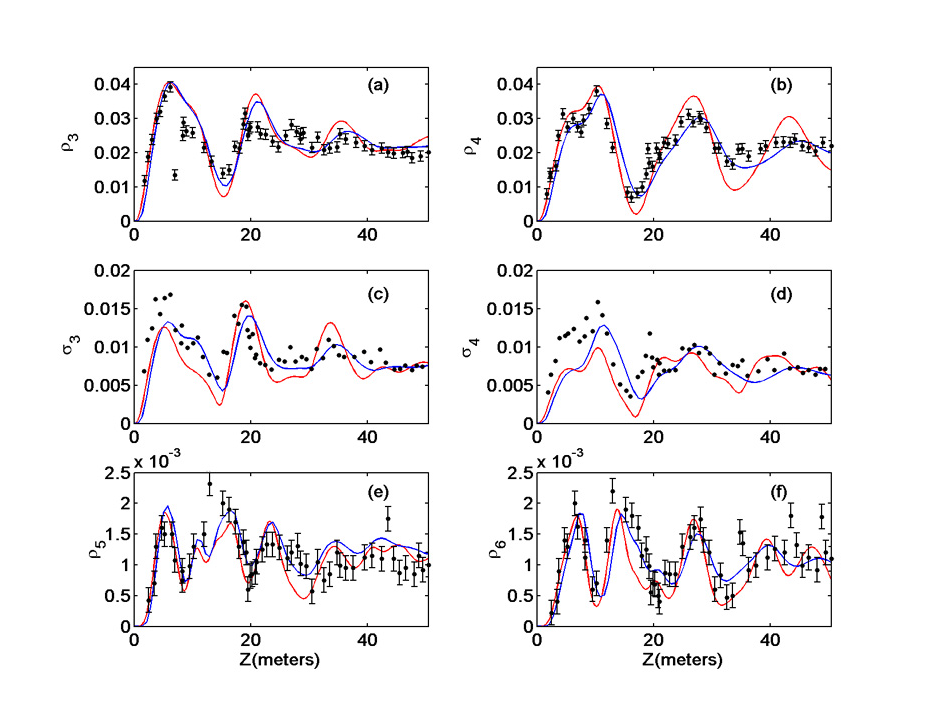
\includegraphics[width=6in]{nlsez55phaseornot.eps}
\end{center}
\renewcommand{\baselinestretch}{1}
\small\normalsize
\begin{quote}
\caption[Figure with caption indented]{This figure caption is indented and single-spaced.  Comparison between the experimental measurements \cite{hart1} (black), the random initial condition NLSE model excluding phase noise (dashed curves) and the stochastic phase noise NLSE model (solid curves) showing the first- and second-order sideband evolution as a function of fiber length for P$_{0} = 5.5$\,W, $\Omega = 366$\,GHz, $\Delta\nu = 0.5$\,GHz, $\gamma = 0.019$\,W$^{-1}$m$^{-1}$, and $\beta^{(2)} = 55$\,ps$^2$/km: dynamical evolution of the: (a) power in the first-order blue-shifted sideband, (b) power in the first-order red-shifted sideband, (c) fluctuations in the first-order blue-shifted sideband, (d) fluctuations in the first-order red-shifted sideband, (e) power in the second-order blue-shifted sideband, (f) power in the second-order red-shifted sideband. \label{fig:fig27}}
\end{quote}
\end{figure} 
\renewcommand{\baselinestretch}{2}
\small\normalsize

The first figure is Fig.\ref{fig:fig27}.   Please note that the figure label should be placed inside the figure caption.  
\newpage

The next figure is placed landscape.  It is Fig.~\ref{fig:mpc}.

\begin{landscape}
\renewcommand{\baselinestretch}{1}
\small\normalsize
\begin{quote}
\begin{figure}
\begin{center}
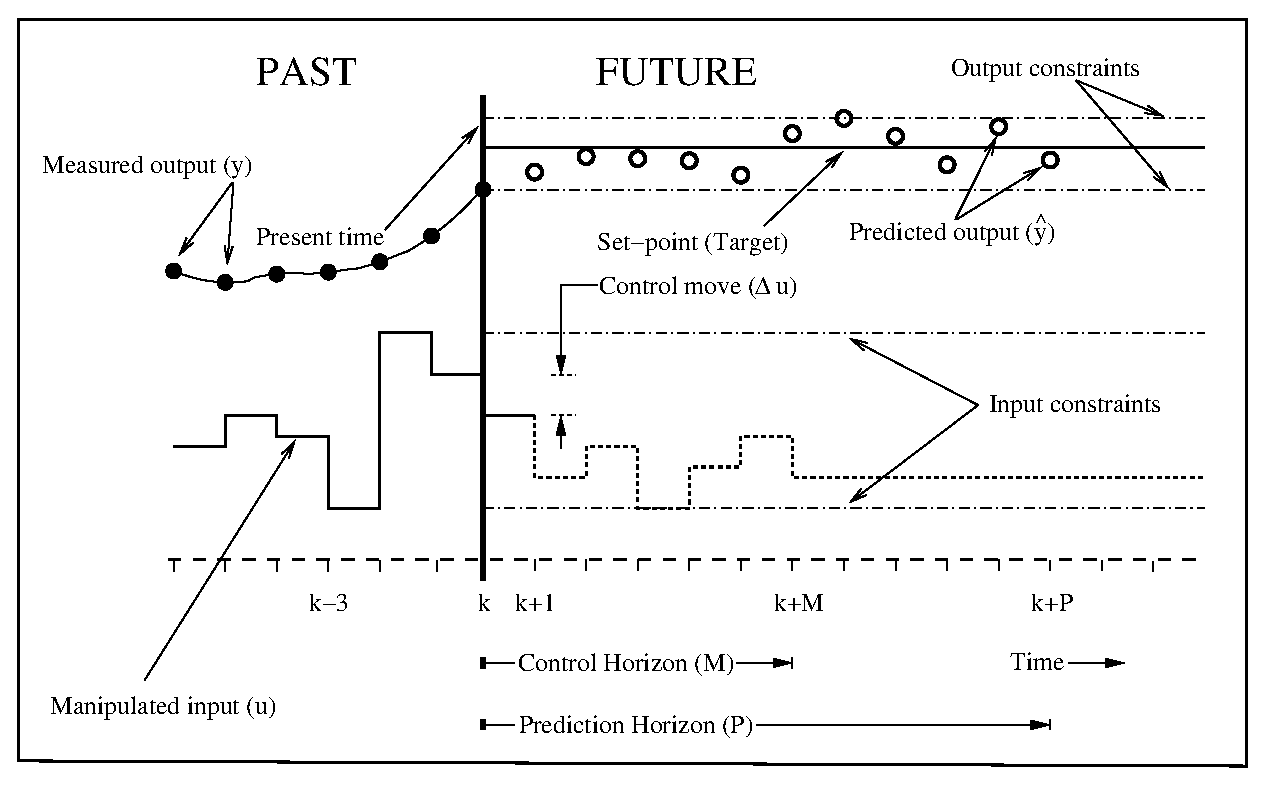
\includegraphics[width=8.2in]{mpc.eps}
\end{center}
\caption{Schematic illustrating receding horizon control.
\label{fig:mpc} }
\end{figure}
\end{quote}
\renewcommand{\baselinestretch}{2}
\small\normalsize
\end{landscape}

This is a my second figure which was placed landscape.  Although I have used the same figure, I have renamed the label to fig:mpc-1.  The second figure now becomes Figure~\ref{fig:mpc-1}.
\begin{landscape}
\renewcommand{\baselinestretch}{1}
\small\normalsize
\begin{quote}
\begin{figure}
\begin{center}
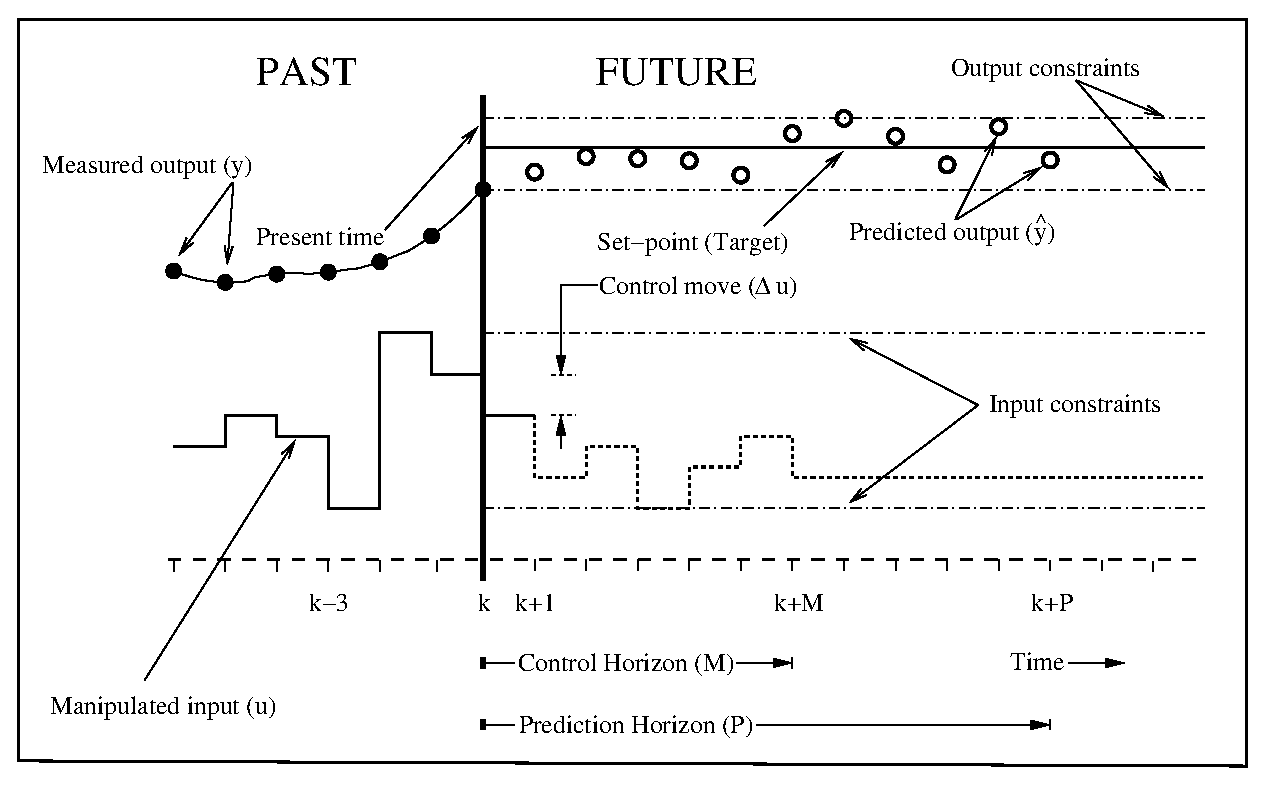
\includegraphics[width=8.2in]{mpc.eps}
\end{center}
\caption[Figure placed landscape on page]{Schematic illustrating receding horizon control. \label{fig:mpc-1}}
\end{figure}
\end{quote}
\renewcommand{\baselinestretch}{2}
\small\normalsize
\end{landscape}

\subsection{Numbering Figures}

If you wish your figures to be numbered 1-100 without any reference to the chapter (e.g., Figure 1.1, 2.1, etc.), change the first line of your mainthesis.tex file to read \begin{verbatim}"\documentclass[12pt]{thesis-2}".\end{verbatim}  

\subsubsection{This is a Subsubsection}

This is my first subsubsection in Chapter 1.


\section[Short Titles]{Short Titles in the Table of Contents, List of Figures, or List of Tables}

The Table of Contents, List of Figures, or List of Tables usually show the entire title of a section, subsection, etc. or table, or the entire caption of a figure.  If you put a short title in square brackets after \begin{verbatim} \section, \table, or \figure, \end{verbatim} the short title will show in your Table of Contents or lists.

\renewcommand{\baselinestretch}{1}
\small\normalsize

\begin{verbatim}
\section[Short Title]{Title of Section} 
\subsection[Short Title]{Title of Subsection} 
\end{verbatim}

or when using a caption in a figure or table
\begin{verbatim}
\caption[Short Caption]{Full text of the caption.}
\end{verbatim}

\renewcommand{\baselinestretch}{2}
\small\normalsize


\section{Figures on Text Page}

Normally figures in the thesis are placed on a page by themselves.  The following figure is placed on the page with text before and after the figure by adding [!!h] after \begin{verbatim} \begin{figure}[!!h] \end{verbatim}.  Please note that the figure label is placed within the caption.

\renewcommand{\baselinestretch}{1}
\large\normalsize

\begin{verbatim}
\begin{figure}[!!h]
 \begin{center}
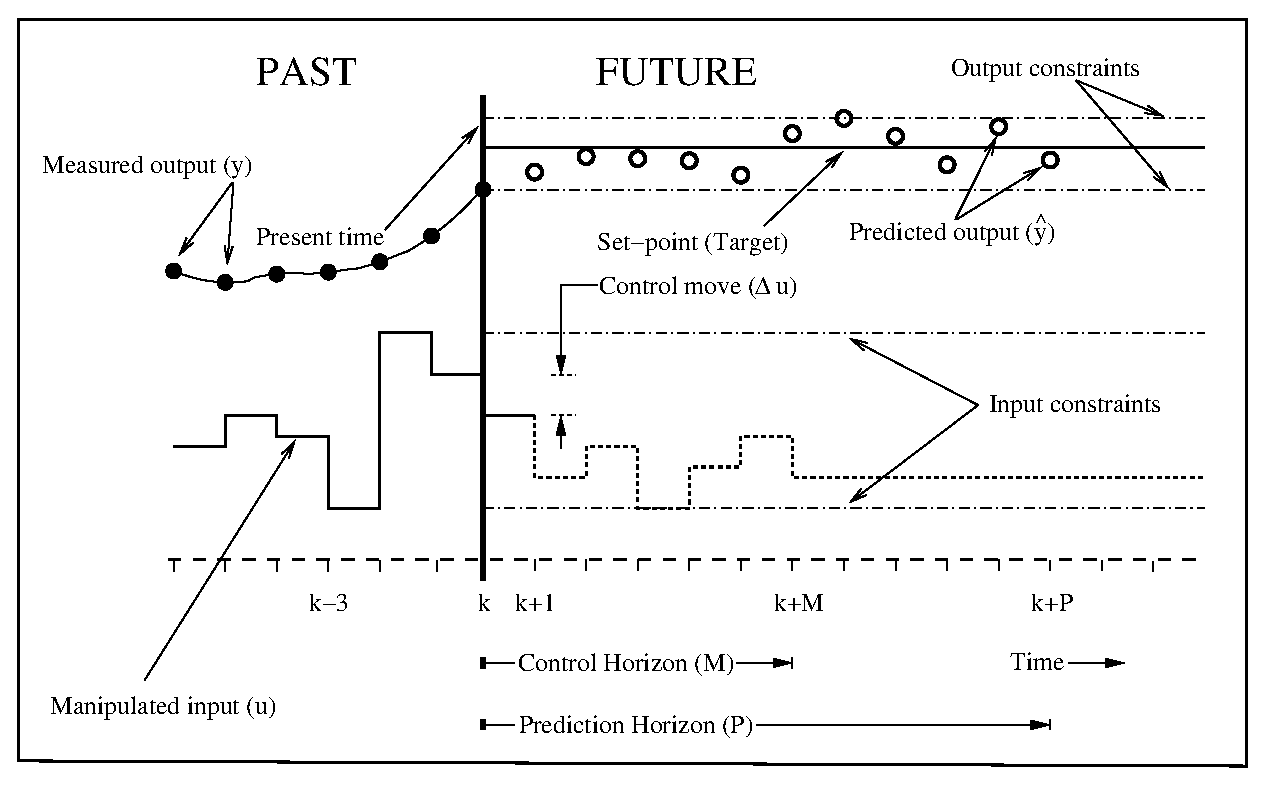
\includegraphics[width=5in]{mpc.eps}
\end{center}
\caption[Short title]{Schematic illustrating receding horizon control.
\label{fig:mpc-2}}
\end{figure}
\end{verbatim}

\begin{figure}[!!h]
 \begin{center}
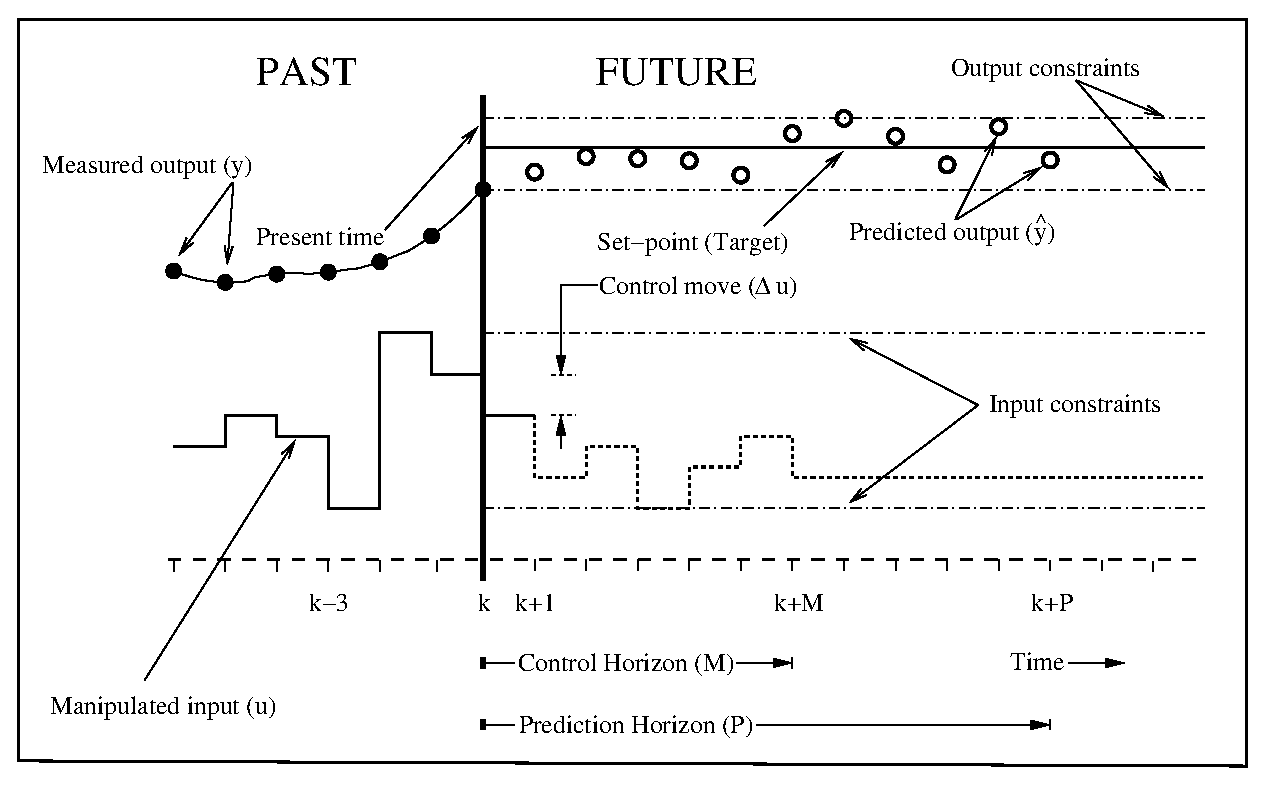
\includegraphics[width=5in]{mpc.eps}
\end{center}
\caption{Schematic illustrating receding horizon control. \label{fig:mpc-2}}
\end{figure}

\renewcommand{\baselinestretch}{2}
\large\normalsize

This does not necessarily mean that the text before and after the figure will be exactly what you want.  Remember Latex will place the figure where it will fit on the page the best.   The previous figure is Figs.~\ref{fig:mpc-2}. 

\section{Wrapping Text around Figure}


\renewcommand{\baselinestretch}{1}
\begin{wrapfigure}{r}{0.4\textwidth}
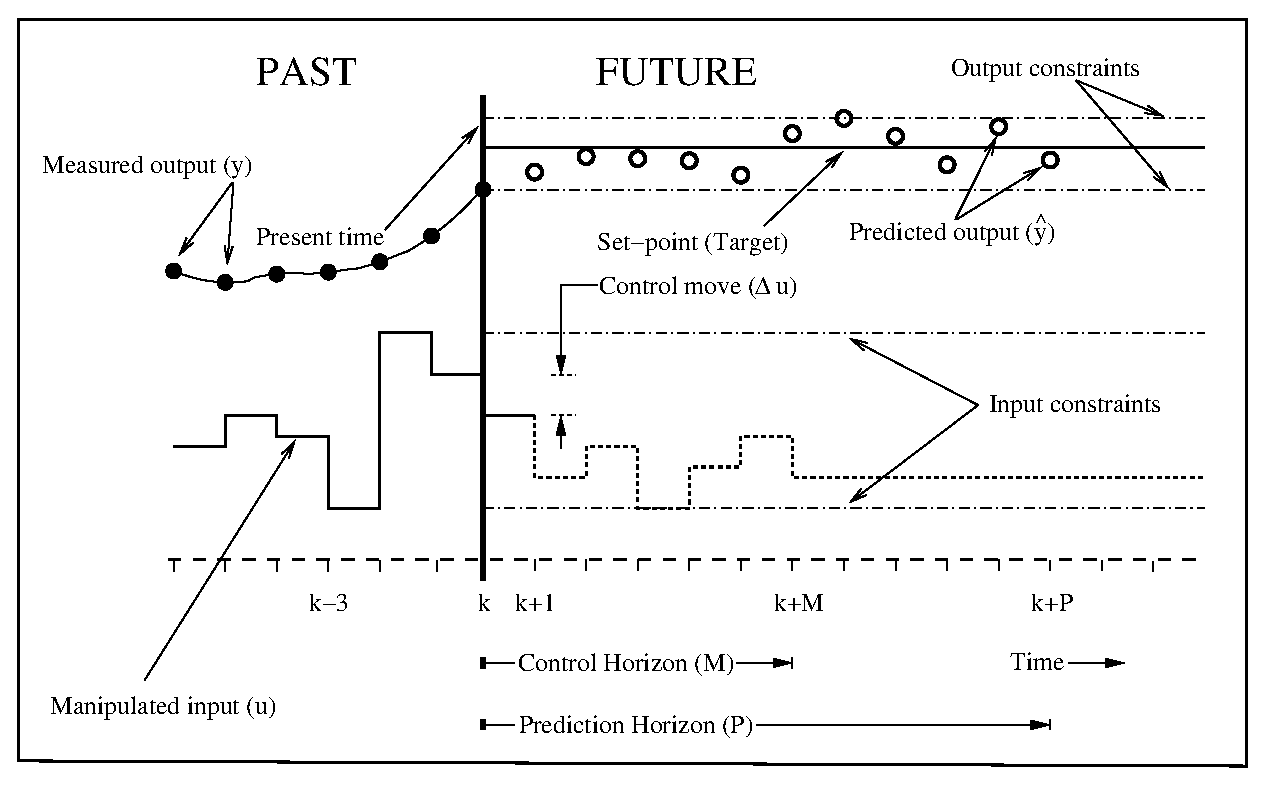
\includegraphics[width=0.4\textwidth]{mpc.eps}
\caption{ Text wrap around figure. \label{fig:test}}
\end{wrapfigure}

\renewcommand{\baselinestretch}{2}
\large\normalsize

By way of summary, at the end of the activity, I reminded the class of what we'd done:  by considering relatively nearby galaxies whose distance we had measured by some other means, we were able to establish a relationship locally between redshift and distance.  
By way of summary, at the end of the activity, I reminded the class of what we'd done:  by considering relatively nearby galaxies whose distance we had measured by some other means, we were able to establish a relationship locally between redshift and distance.  
By way of summary, at the end of the activity, I reminded the class of what we'd done:  by considering relatively nearby galaxies whose distance we had measured by some other means, we were able to establish a relationship locally between redshift and distance.  
By way of summary, at the end of the activity, I reminded the class of what we'd done:  by considering relatively nearby galaxies whose distance we had measured by some other means, we were able to establish a relationship locally between redshift and distance.  See Fig.~\ref{fig:test}.


\section{LaTeX -- A Typesetting Program}

A 13-page explanation of some of the features of LaTeX can be downloaded from http://www.jgsee.kmutt.ac.th/exell/General/LaTeX.html.


\section{Using Bibtex}

Using Bibtex with Latex documents is not difficult.  The bulk of the work is organizing your bibtex file, which is a data base compiled by you of the articles, books, etc. which you use in the bibliographies or reference sections of your publications.  

I have linked several files to this webpage, which will be helpful when you are using Bibtex.  These files can be downloaded from \newline
http://www.ireap.umd.edu/ireap/theses/bibtex.  Please read the file "BibtexInstructions.pdf".  The first two pages explain how to set up and run Bibtex; the remaining pages were taken from a published article and show how the references were cited in the .tex file.   The files BibtexInstructions.tex, Galactic.bib, Dottie.bib are the original .tex files used for BibtexInstructions.pdf.  The file BibtexSamples.tex contains examples of the information needed for the various publications you wish to reference (e.g., articles in refereed journals, books, unpublished articles, conference proceedings, etc.).

If you have questions concerning Bibtex, please contact me at 301-405-4955 or dbrosius at umd.edu.

\section{Using Natbib}

Another option of citing references in the bibliography is using Natbib instead of Bibtex.  You must still create a bibtex file, as noted above.  The command "backslash cite" cannot be used with natbib; instead "backslash citet" and "backslash citep" must be used.    "backslash citet" is used to show reference in the text (e.g., Eq.\ 8 in Reiser,1996 shows ...); "backslash citep" is used in the parenthetical (e.g., Eq.\ 8 (Reiser, 1996) shows ...).  

\begin{verbatim}
Add in preamble -- \usepackage[option]{natbib} 

Add at bottom of mainthesis.tex file --
\bibliography{name of your bibtex file}
\bibliographystyle{plainnat, abbrnat, or unsrtnat}
\end{verbatim}

Typesetting:   Latex, Bibtex, Latex, Latex

The reference sheet for natbib usage can be found at \newline "http://merkel.zoneo.net/Latex/natbib.php".

\section{APS Physical Review Style and Notation Guide}

The following style guide may be downloaded from The American Physical Society at http://forms.aps.org/author/styleguide.pdf:  Physical Review Style and Notation Guide, published by The American Physical Society, compiled and edited by Anne Waldron, Peggy Judd, and Valerie Miller, February 1993.  It may be old, but it is very useful.


% !TEX root = mainthesis.tex
%Chapter 2

\renewcommand{\thechapter}{2}

\chapter{Basic theory of Bose-Einstein condensation}

Bose-Einstein condensation (BEC) is a quantum state of mater in which particles with integer valued spin all tend to occupy or `condense' into the ground state. In dilute gases, condensation occurs when the temperature of the system goes bellow a critical temperature where the bosons become indistinguishable particles and quantum statistics become relevant. 

BECs enable the observation of macroscopic quantum phenomena and there have been a number of fascinating experiments studying the properties of this systems, from measuring interference fringes from a macroscopic wave function to studying collective effects such as the propagation of sound~\cite{ketterle_w._making_1999}, as well as extensive theoretical developments~\cite{dalfovo_theory_1999}. In our experiments however BECs are not the primary object of study, instead they are used as the platform for performing quantum simulations. 

In this Chapter I describe the basic properties of Bose-Einstein condensation in dilute atomic gases. First I will describe the case of an ideal gas and then consider the effects of interactions and a trapping potential. A reader interested in learning about this subject in more depth is advised to read~\cite{Pethick} and~\cite{noauthor_bose-einstein_2003}.

\section{Bose-Einstein condensation of an ideal gas}

At low temperatures and in thermodynamic equilibrium, the mean occupation number of non-interacting identical bosons occupying the state with energy $E$ is given by the Bose distribution
%
\begin{equation}
	n(E_j)=\frac{1}{e^{(E_j-\mu)/k_BT}-1}
	\label{eq:Bose_distribution}	
\end{equation}
%
where $T$ is the temperature, $\mu$ is the chemical potential (the energy cost of adding or removing a particle) and $k_B$ is the Boltzmann constant. In the limit of large temperatures the Bose distribution can be approximated by the Maxwell-Boltzmann distribution
%
\begin{equation}
	n(E_j)\approx e^{-(E_j-\mu)/kT}
\end{equation}
%
which applies to classical, distinguishable particles. The chemical potential is determined by the condition that the total number of particles $N$ is equal to the sum over all states in the distribution $N=\sum_jn(E_j)$ and is therefore a function of $N$ and $T$. Additionally, in order for $n(E_j)$ to be positive definite we must have $\mu\leq E_0$ where $E_0$ is the energy of the ground state. From the Bose distribution we can see that the occupation number of the ground state is unbounded when $\mu\rightarrow0$. As shown in Figure \note{TODO: make figure of Bose distribution} the temperature decreases the occupation number in the ground state increases until all atoms collapse into the lowest energy level and Bose condense. 

\subsection{Critical temperature}
Now I will derive an analytical expression for the critical temperature at which atoms condense. For closely spaced energy levels (compared to $k_B T$) the sum representing the total number of particles can be replaced by the integral
%
\begin{equation}
	N=\int_0^\infty n(E) g(E) dE
	\label{eq:N(E)}
\end{equation}
%
where $g(E)$ is the density of states and $g(E)dE$ corresponds to the number of available states with energy between $E$ and $E+dE$. For a free particle in three dimensions the density of states is
%
\begin{equation}
	g(E)=\frac{V m^{3/2}}{\sqrt{2}\pi^2\hbar^2}E^{1/2},
	\label{eq:free_particle_dos}
\end{equation}
%
and in general the density of states can be expressed as a power of energy $g(E)=C_\alpha E^{\alpha-1}$. 

The integral in Equation~\ref{eq:N(E)} is not analytically solvable, however we can make the simplifying assumption $\mu=0$. The critical temperature $T_c$ is determined by the condition that all particles are in the excited states
%
\begin{align}
	N&=N_{\rm{ex}}(T_c, \mu=0) \nonumber \\
	&=\int_0^{\infty}\frac{g(E)dE}{e^{E/k_BT_c}-1} \nonumber \\
	&= C_\alpha(k_BT_c)^\alpha\int_0^\infty\frac{x^{\alpha-1}}{e^x-1} \nonumber \\
	&= c_\alpha (k_BT_c)^\alpha\Gamma(\alpha)\zeta(\alpha)
	\label{eq:finding_Tc}
\end{align}
%
where I made the substitution $x=E/k_BT_c$, $\Gamma(\alpha)=\int_0^\infty x^{\alpha-1}e^{-x}dx$ is the Gamma function and $\zeta(\alpha)=\sum_{n=1}^\infty n^{-\alpha}$ is the Riemann zeta function. From Equation~\ref{eq:finding_Tc} we find that the critical temperature for Bose-Einstein condensation is
%
\begin{equation}
	k_BT_c=\left(\frac{N}{C_\alpha\Gamma(\alpha)\zeta(\alpha)}\right)^{1/\alpha}.
\end{equation}

As mentioned earlier, Bose-Einstein condensation can be understood in terms of the de Broglie waves associated to particles. The thermal de Broglie wavelength is defined as
%
\begin{equation}
	\lambda_{\rm{th}}=\left(\frac{2\pi\hbar^2}{mk_BT}\right)^{1/2}
\end{equation}
%
and it characterized the spatial extension of the wave packet an individual particle at temperature $T$. Condensation occurs when $\lambda_{\rm{th}}$ becomes comparable with the inter-particle separation $n^{-1/3}$, where $n=N/V$. Using the density of states for a free particle in 3D (Equation~\ref{eq:free_particle_dos})in combination with the expression for the critical temperature (Equation~\ref{eq:finding_Tc}) we find that indeed when $T=T_c$
%
\begin{equation}
	n\lambda_{\rm {th}}^3=\zeta\left(\frac{3}{2}\right)\approx 2.612
\end{equation}
%
both quantities are comparable. The quantity $n\lambda_{\rm{th}}^3$ is known as the phase space density which describes the number of particles contained in a box with volume $\lambda_{\rm{th}}^3$. In order to experimentally produce BECs, a combination of laser and evaporative cooling techniques are deployed such that we can increase the density while minimizing the temperature and therefore maximize the phase space density. The densities for BECs of Alkali atoms typically range in of order $10^{13}$ to $10^{15}$ atoms/cm$^{-3}$.

\subsection{Condensate fraction}

Now we look at the fraction of particles occupying the ground state at temperatures below $T_c$. The total number of particles is given by $N=N_0+N_{\rm{ex}}$. The number of particles in the excited state will be given by the integral in Equation~\ref{eq:N(E)}. For $g(E)=C_\alpha E^{\alpha-1}$and  $\alpha>0$ the integral converges and we get
%
\begin{align}
	N_{\rm{ex}}&=c_\alpha (k_BT)^\alpha\Gamma(\alpha)\zeta(\alpha) \nonumber \\
	&=N\left(\frac{T}{T_c}\right)^\alpha,
\end{align}
%
where I used the expression for the total number of particles at $T_c$ from Equation~\ref{eq:finding_Tc}. The number of particles in the ground state is therefore
%
\begin{align}
	N_0&=N-N_{\rm{ex}} \nonumber \\
	&= N\left[1-\left(\frac{T}{T_c}\right)^\alpha\right]
\end{align}

\subsection{Bose gas in a harmonic trapping potential}

I consider the particular case of particles confined in a three dimensional harmonic potential
%
\begin{equation}
V(\r)=\frac{m}{2}\left(\omega_x^2x^2+\omega_y^2y^2+\omega_z^2z^2\right)
\label{eq:ho}
\end{equation}
%
as it is the most relevant to our experiments that are performed in harmonic traps. The density of states is given by 

\begin{equation}
	g(E)=\frac{E^2}{2\hbar^2\omega_x\omega_y\omega_z},
\end{equation}
%
which corresponds to $\alpha=3$ and $C_3=(2\hbar^3\omega_x\omega_y\omega_z)^{-1}$. Using Equation~\ref{eq:finding_Tc}, the transition temperature is
%
\begin{equation}
 	k_B T_c=\frac{\hbar \bar{\omega}N^{1/3}}{\zeta(3)^{1/3}}\approx0.94\hbar\bar{\omega}N^{1/3}
 \end{equation} 
%
where $\bar{\omega}=(\omega_x\omega_y\omega_z)^{1/3}$ is the geometric mean of the oscillation frequencies. Similarly we find that the condensed fraction is
%
\begin{equation}
	N_0=N\left[1-\left(\frac{T}{T_c}\right)^3\right]
\end{equation}

Condensates in harmonic traps have some striking features that will be further explored in more detail in the following sections. The confining potential makes the BECs both finite sized and inhomogeneous which means that the BEC can be observed both in momentum space and in coordinate space. Another consequence of the inhomogeneity of these systems is the role of two-body interactions, which gets enhanced and leads to noticeable effects in measurable quantities (see~\cite{dalfovo_theory_1999,castin_bose-einstein_1996}).

\section{Bose-Einstein condensation with atomic interactions}

Even though atomic BECs are made from very dilute gases, the system is far from being an ideal gas and interactions need to be taken into account for a complete treatment of the system. 

The collisional properties of particles at low energies, such as cold atoms in a condensate, are dominated by $s$-wave scattering which can be described in terms of a single parameter the scattering length $a$ that determines both the scattering cross section $\sigma=4\pi a^2$ and the . 

The magnitude of the scattering length is determined by the interatomic interaction potentials. For Alkali atoms at large distances, the two-body interactions are dominated by an attractive Van der walls interaction $U(r)=-C_6/r^6$ that arises from dipole-dipole interactions. At smaller distances the attractive potential is replaced by a strong repulsive electron-exchange interaction. This minimal model captures the most important properties of the inter-atomic potential and can be solved analytically~\cite{gribakin_calculation_1993}. 

If the range of the interaction is much shorter than the mean inter-atomic distance the interaction can be approximated by an effective pseudo-potential $U_{\rm{eff}}(\r-\r')$ such that
%
\begin{equation}
	a=\frac{m}{4\pi\hbar^2}\int U_{\rm{eff}}(\r-\r')d \r
\end{equation}
%
which determines
%
\begin{equation}
	U_{\rm{eff}}(\r-\r')=\frac{4\pi\hbar^2a}{m}\delta(\r-\r')=g\delta(\r-\r').
\end{equation}
%
This is a nice approximation as it allows us to model the scattering between atoms as a hard sphere scattering process instead of considering the more complicated inter-atomic potentials. The sign of the scattering length determines the attractive or repulsive nature of the interactions and it  plays an important role in the experimental production of BECs as it determines the rate at which atoms thermalize during evaporative cooling.  For  $\Rb87$ at zero magnetic field $a=103 a_0$ where $a_0=\unit[5.29\times10^{-11}]{m}$ is the Bohr radius while for the more abundant isotope $^85$Rb $a=-\unit[23.44]{nm}$ which means that a BEC with density beyond a critical value can collapse~\cite{gerton_direct_2000}. \note{TODO: try to find references for the values of scattering lengths}

\subsection{Gross-Pitaevskii equation}

The effective Hamiltonian describing $N$ identical bosons with contact interactions can be written as
%
\begin{equation}
	\hat{H}=\sum_{i=1}^N\left[\frac{\mathbf{p}_i^2}{2m}+V(\r_i)\right]+g\sum_{i<j}\delta(\r_i-\r_j),
	\label{eq:many_body_h}
\end{equation}
%
where $V(\r)$ is an external potential and $\mathbf{p}_i=-i\hbar\nabla_i$. We now consider a normalized eigenstate of the Hamiltonian $\Psi(\r_1, \r_2, ..., \r_N)$. We can simplify this state by taking a mean field approach. If we assume that the system has undergone condensation so that the majority of the particles share the same single particle ground state $\psi_0(\r)$ the wavefunction can be approximated by a symmetrized product
%
\begin{equation}
	\Psi(\r_1, \r_2, ..., \r_N)=\prod_{i=1}^N\phi(\r_i),
	\label{eq:mean_field_psi}
\end{equation}
%
where $\psi_0$ is normalized to unity. The energy of the state from Equation~\ref{eq:mean_field_psi} is given by the expectation value
%
\begin{align}
	E&=\int\Psi^*\hat{H}\Psi \,d\r \nonumber \\
	&=N\int\left[-\frac{\hbar^2}{2m}\vert \nabla\phi(\r)\vert^2+V(\r)\vert\phi(\r)\vert^2+\frac{(N-1)}{2}g\vert \phi(\r)\vert^4\right]d\r,
	\label{eq:mean_field_E}
\end{align}
%
where $N(N-1)/2\approx N^2/2$ is counting the number of terms in the interaction energy. Now we introduce the wave function of the condensate $\psi(\r)=N^{1/2}\phi(\r)$, which when inserted in Equation~\ref{eq:mean_field_E} makes the $N$ factors disappear. The optimal form of $\psi$ should minimize the energy subject to the normalization condition $N=\int\vert\psi(\r)\vert^2\,d\r$. This can be done by introducing a Lagrange multiplier $\mu$
%
\begin{align}
	\frac{\delta}{\delta \psi^*(\r)}\left(E-\mu\int\vert\psi\vert^2\,d\r \right) 
	&= \left[-\frac{\hbar^2}{2m}\nabla^2+V(\r)+g\vert\psi(\r)\vert^2-\mu\right]\psi(\r)
	=0
\end{align}
%
and we thus find that the condensate wave function obeys a non-linear Schr\"odinger equation known as the Gross-Pitaevskii (GP) equation
\footnote{The GP equation is very minimally relevant to my experiment but it still feels good knowing where it comes from.}.  
%
\begin{equation}
	\left[-\frac{\hbar^2}{2m}\nabla^2+V(\r)+g\vert\psi(\r)\vert^2\right]\psi(\r)=\mu\psi(\r)
\end{equation}
%
where $\mu$ plays the role of the chemical potential. The dynamics of the condensate will similarly be described by the time-dependent GP equation
%
\begin{equation}
	i\hbar\frac{\partial}{\partial t}\psi(\r,t)=\left[-\frac{\hbar^2}{2m}+V(\r)+g\vert\psi(\r,t)\vert^2\right]\psi(\r,t)
\end{equation}

The GP equation describing the relevant phenomena associated
with BECs, for example the propagation of collective excitations and the expansion of the condensate when released from a trap. The crucial assumption when deriving these equations was the mean field approximation which should be valid for dilute BECs in which the condensate fraction is close to unity. The excitations of the system (deviations from the mean field) can be treated using Bogoliubov theory for weakly interacting bosons\cite{Pethick}. 

\subsection{Thomas-Fermi approximation}

For systems with large $N$, the interaction term in the GP equation is very large compared to the kinetic energy\footnote{It can be shown that the ratio of kinetic energy to interactions scales like $N^{-4/5}$}. As the kinetic energy becomes less important we enter the Thomas-Fermi (TF) regime where the energy of the system is given only by the external potential and the mean field energy and the GP equation is considerably simplified 
%
\begin{equation}
	\left[V(\r)+g\vert\psi(\r)\vert\psi(\r)\vert^2\right]\psi(\r)=\mu\psi(\r).
\end{equation}
%

In the TF regime the density distribution of the condensate $n(\r)=\vert\psi(\r)\vert^2$ reflects the shape of the external potential
%
\begin{equation}
	n(\r)=g^{-1}[\mu-V(\r)],
\end{equation}
%
when $\mu-V(\r)>0$ and is otherwise zero. For a harmonic confining potential (Equation~\ref{eq:ho}) as is typical in our experiments we find that the length scale that characterizes the size of the condensate is the Thomas-Fermi radius
%
\begin{equation}
	R_j=\sqrt{\frac{2\mu}{m\omega_j^2}}, \ \ \ j=x,y,z.
\end{equation}
%
The density of the condensate is described by an inverted parabola
%
\begin{equation}
	n(\r)=\frac{\mu}{g}\left(1-\frac{x^2}{R_x^2}-\frac{y^2}{R_y^2}-\frac{z^2}{R_z^2}\right).
	\label{eq:n_tf}
\end{equation}
 %
 
By integrating over Equation~\ref{eq:n_tf} we find that
 %
 \begin{equation}
 	N=\frac{8\pi}{15}\frac{\mu}{g}R_xR_yR_z,
 \end{equation}
 %
 which is a useful quantity for determining the number of atoms in the condensate based on density profiles. In practice our images are taken after the atoms are released from the trap and the density profile is modified due to interactions. This will be discussed in more detail in the next following section. 

\section{Density distributions}

Most ultracold atoms experiments are probed by directly imaging the atoms (e.g. with absorption imaging, Section~\ref{sec:absorption imaging}). If the atoms are imaged in-situ we gain access to their spatial density profiles. If the atoms are released from the trap and allowed to expand in time of flight (TOF) we can measure their momentum distribution. In this section I summarize the signatures in the density distributions of BECs and thermal atoms confined in a harmonic potential both in-situ and after TOF. 

For a thermal gas in a harmonic potential at temperatures higher than the level spacing $k_BT>\hbar\omega_{x,y,z}$ the density is given by~\cite{ketterle_w._making_1999}
%
\begin{equation}
	n_{\rm{th}}(\r)=\frac{1}{\lambda_{\rm{th}}^3}g_{3/2}(z(\r))
\end{equation}
%
where $z(\r)=\exp(\mu-V(\r)/\k_BT$, $V(\r)$ is given by Equation~\ref{eq:ho}, $\mu$ is the chemical potential and $g_j(z)=\sum_iz^i/i^j$ is the Bose function. The Bose function introduces effects of quantum statistics and compared to a distribution of distinguishable particles, the peak density of a Bose gas is increased by $g_{3/2}(z)/z$, a phenomenon known as Bose-enhancement.

The distribution after TOF can be calculated considering that the trapped atoms fly ballistically from their position in the trap. An atom starting initially at the point $\r_0$ moves to the point $\r$ after a time $t$ if its momentum is given by $\mathbf{p}=m(\r-\r0)/t$, and it can be shown that
%
\begin{align}
	n_{\rm{tof}}&=\frac{1}{\lambda_{\rm{th}}}\prod_{i=1}^3g_{3/2}\left(\exp\left[\mu-\frac{m}{2}\sum_{i=1}^3x_i^2\left(\frac{\omega_i^2}{1+\omega_i^2t^2}\right)\right]\right) \nonumber \\
	&\approx \frac{1}{\lambda_{\rm{th}}}g_{3/2}\left(\exp\left[(\mu-\frac{mr^2}{2t^2})/k_BT\right]\right)
\end{align}
%
where the approximation in the second line is valid for $t\gg \omega_i^{-1}$. The temperature of the atoms can be estimated by looking at the wings of the density distribution after TOF. Even with the case of Bose enhancement, the density of the wings still decays exponentially as $\exp(-x_i^2/\sigma_i^2)$ and the temperature of the cloud can be determined using
%
\begin{align}
	k_BT&=\frac{m}{2}\left(\frac{\omega_i^2}{1+\omega_i^2t^2}\sigma_i^2\right) \nonumber \\
	&\approx \frac{m}{2}\left(\frac{\sigma_i}{t}\right)^2
\end{align}

For the case of a BEC at zero temperature (no thermal fraction) the in-situ density distribution is described by the Thomas-Fermi distribution 
%
\begin{align}
	n(\r)&=n_0\left(1-\frac{x^2}{R_x^2}-\frac{y^2}{R_y^2}-\frac{z^2}{R_z^2}\right) \nonumber \\  
	&= \frac{15N}{8\pi R_xR_yR_z}\left(1-\frac{x^2}{R_x^2}-\frac{y^2}{R_y^2}-\frac{z^2}{R_z^2}\right) .
\end{align}

Even though the BEC is in the motional ground state, it will expand during TOF as a consequence of interactions. The expansion can be determined using the time dependent GP equation. A detail account of the procedure can be found in \cite{castin_bose-einstein_1996}, the procedure relies on using the ansatz that the TF radii expand as
%
\begin{equation}
	R_i(t)=\lambda_i(t)R_i(t=0),
	\label{eq:castin_dum_radius}
\end{equation}
%
where I assumed that the condensate is in the trap at $t=0$ which implies that $\lambda_i(0)=1$. If the trap is suddenly turned off at $t>0$ from inserting the TF wave function with radii given by Equation~\ref{eq:castin_dum_radius} into the time-dependent GP equation we find a series differential equations
%
\begin{equation}
	\frac{d^2\lambda_i}{dt^2}=\frac{\omega_i^2}{\lambda_i\lambda_x\lambda_y\lambda_z}
\end{equation}
%
which can be used to determine the density profile of the BEC in TOF. Alternatively if the density profile of the BEC is known from an image, these relations can used to back-propagate what the original TF radii of the confined condensate was. 

For partially condensed clouds the density profiles will be given by a combination of the thermal density profiles and the Thomas-Fermi density profile. 




% were when the condensate
% was confined.
% or by measuring the
% TOF radii via absorption imaging, back-propagate what the original radii were when the condensate
% was confined.
% %
% \begin{align}
% 	n(\r)&=n_0e^{-(\frac{x^2}{2\sigma_x^2}+\frac{y^2}{2\sigma_y^2}+\frac{z^2}{2\sigma_z^2})}\nonumber \\
% 	&= \frac{15N}{8\pi R_xR_yR_z},
% \end{align}
% %
% where $\sigma_i=\omega_i^{-1}\sqrt{k_BT/m}$. Using the equipartition theorem we find that the spatial extension of the cloud and the temperature are related by 
% %
% \begin{equation}
% 	T=\frac{m}{k_B}\sigma_i^2\omega_i^2
% \end{equation}

% \note{TODO: what is my chemical potential?}


% For a given trapping potential $U(\r)$, the density distribution of a thermal ensamble is
% \begin{equation}
% 	n(\r) = n_0 e^{-\frac{U(\r)}{k_BT}}.
% \end{equation}
% %
% The temperature $T$ can be derived from the density distribution. For a 3D harmonic trap


% !TEX root = mainthesis.tex

%Chapter 3


\renewcommand{\thechapter}{3}

\chapter{Manipulation and detection of ultra-cold atoms}
\label{ch:Ch3}

All of the experiments described in this thesis were performed using ultracold clouds of $\Rb87$. Both the cooling and trapping of atoms as well as the engineering of interesting potentials and detection of atoms rely on the interaction of atoms with electromagnetic fields as well as with static and oscillating magnetic fields. 

In this Chapter I describe the techniques and interactions that make our experiments possible. This Chapter is not meant to be an extensive survey of atomic physics but rather covers the topics that are most relevant to the experiments presented in this thesis. The references I included are helpful if the reader is interested in the details of the derivations or wants to expand on a given topic. I start by describing the electronic structure of $\Rb87$. Then I review the interactions of atoms with magnetic fields which allows us to shift the energies of different atomic states. I describe the foundations of atom-light interactions that make possible both laser cooling and trapping of atoms and gives rise to Raman induced transitions. Finally I discuss the absorption imaging technique that we use to detect atoms after all our experiments are performed. 

\section{Electronic structure of $^{87}$Rb}
\label{sec:electronic_structure}

Rb is an Alkali metal (also Li, which exists in our vacuum chamber but was never used). Alkali metals correspond to the first group (leftmost column) of the periodic table and are characterized by having a single valence electron, which makes the description of their internal structure much simpler than that of other elements. We can describe the state of an electron in an atom by its angular momentum $\mathbf{\hat{L}}$ and its spin $\mathbf{\hat S}$. Because of Pauli's exclusion principle there can not be two electrons with the same quantum numbers and in multi-electron atoms they tend to fill `shells' of different angular momentum values, historically labeled by the letters $S,\ P,\ D,\ F,\ ...$\footnote{This terms were used to describe the lines in the emission spectra when they were first discovered. $S$ stands for sharp, $P$ for principal $D$ for diffuse and $F$ for further noted} (corresponding to $L=1,\ 2,\ 3,\ 4,\ ...$). In particular Rb has 4 filled shells and one electron in the $5S$ 
shell, where the number $5$ corresponds to the principal quantum number $n$. Figure \note{TODO: make figure of atomic energy levels} shows the energy levels of the ground state $5S$ and its closest $5P$ orbital. %In the absence of interactions, the $m_l$ sublevels within an orbital are degenerate.

The atomic level structure is modified by relativistic effects. In particular the relativistic treatment of the electron's motion gives rise to an interaction between the electron's intrinsic magnetic moment (the spin) $\mathbf{\hat S}$ and the orbital angular momentum $\mathbf{\hat L}$. This spin-orbit coupling interaction $\hat H_{\rm {fs}} \propto \mathbf{L}\cdot\mathbf{S}$ causes the fine structure splitting of the electronic orbitals into levels with different total electronic angular momentum $\mathbf{J}=\mathbf{\hat L}\cdot\mathbf{\hat S}$. Figure~\ref{fig:fs_hfs}b show the $5^2S_{1/2}$, $5^2P_{1/2}$ and $5^2P{3/2}$ electronic configurations that arise from this splitting, where the subscript indicates the value of $J$. For $S$ ($L=0$) orbitals $J=1/2$ is the only possible value and the levels are not split. For the $P$ orbital ($L=1$) $J$ and a single electron with $S=1/2$, $J$ can be $1/2$ or $3/2$ and the $P$ orbital splits into two levels. The $5S_{1/2}\rightarrow 5P_{1/2}$ is known as the D1 line and has wavelength $\lambda=\unit[794.979]{nm}$ and $5S_{1/2}\rightarrow 5P_{3/2}$ transition is known as the D2 line and has $\lambda=\unit[790.241]{nm}$ \cite{Steck}. 

The atomic level structure gets further modified by the magnetic interaction of the electronic magnetic flux density with the nuclear spin $\mathbf{I}$. This is another kind of spin-orbit interaction that gives rise to the hyperfine splitting of the atomic levels which can be described by the Hamiltonian $\hat H_{\rm{hfs}} = A_{\rm{hfs}}\mathbf{I}\cdot\mathbf{J}$. A complete derivation of $\hat H_{\rm{hfs}}$ can be found in~\cite{schwartz_theory_1955}. The hyperfine levels correspond to different values of the total angular momentum $\hat F=\hat J+\hat I$. For $\Rb87$ $I=3/2$~\cite{Steck} which results in the level structure shown in Figure~\ref{fig:fs_hfs}c 

\note{TODO: talk about cooling and repumping transitions which is relevant for the absorption imaging section.}

\section{Interaction between atoms and magnetic fields}
\label{sec:zeeman_effect}

Atoms have have an intrinsic magnetic moment that is given by the sum of nuclear and electronic moments
%
\begin{equation}
	\boldsymbol{\hat \mu}=-\frac{g_J\mu_B}{\hbar} \mathbf{\hat J}+\frac{g_I\mu_N}{\hbar}\mathbf{\hat I}=\frac{\mu_B g_F}{\hbar} \mathbf{\hat F}
\end{equation}
%
where $\mu_B$ is the Bohr magneton, $\mu_N$ \footnote{$\mu_N\ll\mu_B$ and therefore $\boldsymbol{\hat \mu}\approx-\mu_Bg_J/\hbar\mathbf{\hat J}$} is the nuclear magneton and $g_J$, $g_I$ and $g_F$ are the Land\'e $g$-factors corresponding to the electronic, nuclear and total angular momentum. In the presence of an external magnetic field $\mathbf B$, the internal levels of an atom get modified due to the Zeeman~\cite{Zeeman_effect} interaction
%
\begin{equation}
	\hat{H}_{\rm{Zeeman}}=-\boldsymbol{\hat \mu}\cdot\mathbf{B}
	\label{eq:zeeman_hamiltonian}
\end{equation}
%
which has the effect of lifting the degeneracy of the different $m_F$ states. We take advantage of this effect for making (state-dependent) magnetic traps for the atoms by using magnetic field gradients and for the experiments presented in Chapters~\ref{ch:Fourier_spectroscopy},~\ref{ch:clock_states} and \ref{ch:Rashba} the shifts in the $m_F$ energies allowed us to treat each state as a pseudospin that we then coherently manipulated using the techniques described in Section~\ref{sec:quantum_coherent_dynamics}.

The total energy shifts are calculated by diagonalizing the full atomic Hamiltonian including the fine and hyperfine structure terms. For a small magnetic field the Zeeman term can be treated as a perturbation and the energy split is linear with the magnitude of the field $\Delta E_{\rm{Zeeman}}=g_F\mu_B m_FB$, what is known as the `linear Zeeman regime' where $F$ and $m_F$ are good quantum numbers. In contrast, in the `Pachen-Back regime' large magnetic fields the Zeeman term dominates over the fine and hyperfine terms and therefore the good quantum numbers of the system are $J$ and $m_J$. Our experiments typically operate in an intermediate regime ($B\sim 10-30\,\rm{G}$)energies where the magnetic field and as a result the energy of $m_F=0$ gets a small shift in energy that is quadratic in $B$. For atoms in $F=1$ we define this quadratic Zeeman shift as $\epsilon=E_0-(E_{+1}-E_{-1})/2$, where $E_{m_F}$ is the Zeeman shift for state $m_F$.

For the particular case of $J=1/2$ (like the ground state of Alkalis) the Zeeman energies can be found analytically using the Breit-Rabi formula~\cite{breit_measurement_1931}
%
\begin{equation}
	E_{m_F}=-\frac{1}{2(2I+1)}+\frac{\mu_Bg_Im_FB}{\Delta E_{\rm{hf}}}+\frac{1}{2}\sqrt{1+\frac{4m_F}{2I+1}x+x^2},
	\label{eq:Breit_rabi}
\end{equation}
%
where $\Delta E_{\rm{hf}}=A_{\rm{hf}}(J+1/2)$ and $x=(g_J-g_I)\mu_B B_z/\Delta E_{\rm{hf}}$. Figure \note{TODO:make figure} shows the energies of the $m_F$ levels for the $F=1$ and $F=2$ manifolds of $\Rb87$.

\section{Interaction between atoms and electric fields}
\label{sec:atom-lignt_interactio n}

In this section I will discuss the interaction between atoms and electromagnetic radiation (light). After laying the foundations I will discuss applications using off-resonant light such as optical dipole traps and Raman transitions. I will not cover laser cooling which has been covered extensively in the literature~\cite{metcalf_deceleration_1999,phillips_nobel_1998} and PhD theses from previous lab members~\cite{CampbellThesis,PriceThesis}. 

In the presence of an electric field $\mathbf E$ an atom can become polarized and therefore its energy levels get modified by the Stark effect~\cite{stark_beobachtungen_1914}. If the electric field is spatially uniform with respect to the atom's size we consider the electric field as a classical object and its effect on the atom can be described by the the Hamiltonian~\cite{Cohen-Tanoudji}  
%
\begin{equation}
\hat{H}_{\rm{dip}} = -\mathbf{\hat d}\cdot\mathbf{E},
\label{eq:dipole_ham}	
\end{equation}
%
where $\mathbf{\hat d}=-e\sum_j r_j$ is the atomic dipole operator, $e$ is the electron charge and $\hat r_j$ are the position operators of the atom's electrons relative to the center of mas of the atom. This approximation, known as the dipole approximation, is valid for electromagnetic radiation when the wavelength is much larger than the size of an atom $\lambda\gg r_{\rm{atom}}$~\cite{SteckTextbook}. 

For a coherent electromagnetic field $\mathbf{E}(\omega,t)$ with angular frequency $\omega$, the dipole Hamiltonian can be written in terms of a dynamic polarizability
%
\begin{equation}
	\hat{H}_{\rm{dip}}=-\alpha_{\mu\nu}(\omega)E_{\mu}^{(+)}E_{\nu}^{(-)}
\end{equation}
%
where $\mathbf{E}^{(\pm)}$ are the possitive/negative frequency components of the field. $\alpha_{\mu\nu}(\omega)$ can be found by looking at the (time averaged) shift in the energy of the a given state state using second order time-dependent perturbation theory~\cite{SteckTextbook,deutsch_quantum_2010}. For the ground state $\ket{g}$ the polarizability takes the form
%
\begin{equation}
	\alpha_{\mu\nu}(\omega)=\sum_j\frac{2\omega_{jg}\bra{g}d_\mu\ket{e_j}\bra{e_j}d_\nu\ket{e_j}}{\hbar(\omega_{jg}^2-\omega^2)},
\end{equation}
%
where $\ket{e_j}$ represent the excited states and $\omega_{jg}=(E_j-E_g)/\hbar$. The dipole operator is a rank-1 tensor and can be represented by 3 irreducible tensor operators\footnote{A rank $k$ tensor can be represented by $2k+1$ irreducible tensor operators, which are collection of operators that transforms under
rotations like the spherical harmonics $Y_{kq}(\theta, \phi)$} (see~\cite{SteckTextbook} for a complete derivation). In the limit of small magnetic fields so that $F$ and $m_F$ are good quantum numbers describing the state of the atom $\ket{n, F, m_F}$ the dipole Hamiltonian in this representation takes a convenient form
%
\begin{align}
	\hat{H}_{\rm{dip}}= &\alpha^{(0)}(\omega)(\mathbf{E}^{(-)}\cdot\mathbf{E}^{(+)}) 
	+\alpha^{(1)}(\mathbf{E}^{(-)}\times\mathbf{E}^{(+)})\cdot\mathbf{\hat{F}}  \nonumber \\ 
	&+ \alpha^{(2)}E_i^{(-)}E_j^{(+)}	\left(\frac{1}{2}(F_iF_j+F_jF_i)-\frac{1}{3}\mathbf{\hat F}^2\delta_{i,j}\right)\Big],
	\label{eq:light_matter_coupling}
\end{align}
%
where $\alpha^{(0)}$, $\alpha^{(1)}$ and $\alpha^{(2)}$ are the scalar, vector and tensor polarizabilities respectively and $\hat{\mathbf{F}}$ is the total angular momentum operator. For all our experiments $\alpha^{(2)}$ is very small so I will limit the discussion to the effect of the first two terms. The scalar term is responsible for the dipole force that allow us to trap atoms using off-resonant light and the vector component is necessary for engineering spin-orbit coupling through Raman transitions and other spin-dependent potentials. 

\subsection{Scalar polarizability}
\label{sec:scalar_light_shift}

The scalar polarizability takes the form
%
\begin{equation}
	\alpha^{(0)}=\sum_j\frac{2\omega_{jg}\bra{g}\mathbf{d}\cdot\hat{\epsilon}\ket{e_j}\vert^2}{\hbar(\omega_{jg}^2-\omega^2)},
\end{equation}
%
where $\hat{\epsilon}$ represents the polarization vector of the light. The matrix element can be expressed in terms of the Clebsch-Gordan coefficients and the reduced matrix element using the Wigner-Eckart theorem~\cite{Sakurai}. For the ground state of an Alkali atom ($J=1/2$) the expression above gets simplified to
%
\begin{equation}
	\alpha^{(0)}\approx\sum_{J'}\frac{2\omega_{JJ'}\vert\langle J=1/2 \| \mathbf{d}\|J'\rangle\vert^2}{3\hbar(\omega_{JJ'}^2-\omega^2)}.
\end{equation}

The dipole matrix elements needed to compute the polarizability are related to the transition scattering rate via Fermi's golden rule~\cite{Sakurai,SteckTextbook}
\begin{equation}
	\Gamma_{JJ'}=\frac{\omega_{JJ'}^2}{3\pi\epsilon_0\hbar c^3}\frac{2J+1}{2J'+1}\vert\langle J \| \mathbf{d}\|J'\rangle\vert^2,
\end{equation}
%
and combining this with the expression for the intensity of the electric field $I(\r)=2\epsilon_0c\vert \mathbf{E}(\r)\vert^2$ it can be shown that for linearly polarized light the energy of the ground state manifold is shifted by
\begin{equation}
	U(\omega,\r)=-\frac{\pi c^2 I(\r)}{2}\left[ \frac{\Gamma_{\rm{D1}}}{\omega_{\rm{D1}}^2}\left(\frac{1}{\omega+\omega_{\rm{D1}}}-\frac{1}{\omega-\omega_{\rm{D1}}}\right)+\frac{2\Gamma_{\rm{D2}}}{\omega_{\rm{D2}}^2}\left(\frac{1}{\omega+\omega_{\rm{D2}}}-\frac{1}{\omega-\omega_{\rm{D2}}}\right)\right],
\end{equation}
%
where only the the most significant contribution from the closest transitions  (the D1 and D2 lines) are included. Here $U(\r)$ is related to the real part of the polarizability which is in fact a complex valued number. So far I have only considered the real part by assuming the excited states have an infinitely long lifetime. However, in reality the atom can spontaneously emit photons and decay. This exponential decay can be accounted for by adding an imaginary contribution to the energies $\omega_D\rightarrow\omega_D+i\Gamma_D\omega^3/\omega_D^3$ of the D1 and D2 transitions~\cite{grimm_optical_2000}. The scattering rate is related to the imaginary part of the polarizability and is given by
%
\begin{equation}
	\Gamma(\omega,\r)=\frac{\pi c^2I(\r)}{2\hbar}\left[ \frac{\Gamma_{\rm{D1}}\omega^3}{\omega_{\rm{D1}}^6}\left(\frac{1}{\omega+\omega_{\rm{D1}}}-\frac{1}{\omega-\omega_{\rm{D1}}}\right)^2+\frac{2\Gamma_{\rm{D2}}\omega^3}{\omega_{\rm{D2}}^6}\left(\frac{1}{\omega+\omega_{\rm{D2}}}-\frac{1}{\omega-\omega_{\rm{D2}}}\right)^2\right]
	\label{eq:scattering}
\end{equation}

The energy shift $U(\omega,\r)$ is a conservative term and is related to dipole trapping while the scattering term $\Gamma(\omega,\r)$ is dissipative and is important for laser cooling. In the context of engineering potentials for ultracold atoms with off-resonant light, the scattering is translated into heating because every time an atom emits a photon with angular frequency $\omega_L$ it gets a recoil momentum $\hbar\k_L$.  

If the frequency $\omega$ satisfies the relation $\omega+\omega_{\rm D}\gg\omega-\omega_{\rm D}$ we can neglect the terms proportional to $1/(\omega+\omega_{\rm D})$, an approximation typically known as the rotating wave approximation (RWA). If the RWA is valid then the frequency dependence of both the energy shifts and the scattering rates will be given by the detuning from the D1 and D2 transitions. 

\subsubsection{Optical trapping}
One important application of the scalar light-shift is to create optical traps for our clouds of ultracold atoms. The use optical fields with non-uniform spatial intensity can generate traps (and anti-traps) for the atoms which experience a force proportional to the intensity gradient $F_{\rm{dip}}=-\nabla U(\r)$.  \note{TODO: make nice figure of dipole trap?}. The production of BECs in our lab relies on the use of focused Gaussian laser beams with $\lambda=\unit[1064]{nm}$.  The intensity profile of a focused Gaussian beam propagating along $\ez$ is given by 
%
\begin{equation}
 	I(x,y,z) = \frac{2P}{\pi\omega^2(z)}e^{-\frac{x^2+y^2}{\omega^2(z)}}
 \end{equation} 
 %
 where $P$ is the total power of the beam and the $1/e^2$ radius is given by $w(z)=w_0\sqrt{1+z^2/z_R^2}$ where the minimum radius $w_0$ is known as the waist and $z_R=\pi\omega_0^2/\lambda$ is the Rayleleigh range. If the extent of an atomic cloud is small compared to the size of the beam we can perform a Taylor expansion around $\r=0$ to obtain the trapping potential
 %
 \begin{equation}
 	U(\r) = -U_0\left(1-2\frac{x^2+y^2}{\omega_0^2}-\frac{z^2}{z_R^2}\right).
 \end{equation}
%
The oscillation frequencies of the trap along the radial direction are $\omega_r=(4U_0/m\omega_0^2)^{1/2}$ and along the axial direction $\omega_z=(2U_0/mz_R)^{1/2}$. The beam waist is usually much smaller than the Rayleigh range ($\omega_0\sim \unit[50-150]{nm}$ for my experiments) and therefore the trap is much stronger along the axial direction. To get around this we use a `crossed dipole trap' which is formed by a combination of two cross-polarized\footnote{The beams are cross-polarized to avoid interference between them} focused Gaussian beams propagating along perpendicular axes, ensuring that we get good confinement of atoms along all spatial directions. 

For a given trapping potential $U(\r)$, the density distribution of a thermal ensamble is
\begin{equation}
	n(\r) = n_0 e^{-\frac{U(\r)}{k_BT}}.
\end{equation}
%
The temperature $T$ can be derived from the density distribution. For a 3D harmonic trap
%
\begin{equation}
	n(\r)=n_0e^{-(\frac{x^2}{2\sigma_x^2}+\frac{y^2}{2\sigma_y^2}+\frac{z^2}{2\sigma_z^2})},
\end{equation}
%
where $\sigma_i=\omega_i^{-1}\sqrt{k_BT/m}$. Using the equipartition theorem we find that the spatial extension of the cloud and the temperature are related by 
%
\begin{equation}
	T=\frac{m}{k_B}\sigma_i^2\omega_i^2
\end{equation}

\note{TODO: figure of dipole traps}

\note{TODO: talk about magic wavelength}

\subsection{Effective magnetic fields from vector polarizability}
\label{sec:}

Recall the Zeeman Hamiltonian introduced in Section~\ref{sec:zeeman_effect}. The term proportional to the vector polarizability in Equation~\ref{eq:light_matter_coupling} looks very similar to Equation~\ref{eq:zeeman_hamiltonian} for an effective magnetic field
%
\begin{equation}
	\mathbf{B}_{\rm{eff}}=-\frac{i\hbar}{\mu_Bg_J}\alpha^{(1)}(\mathbf{E}^*\times\mathbf{E}).
\end{equation}

For Alkali atoms the vector poarizability takes the form
%
\begin{equation}
	\alpha^{(1)}= \frac{2\alpha^{(0)}\Delta_{\rm{fs}}}{3(\tilde{E}-\hbar\omega)}
\end{equation}
%
where $\Delta_{\rm{fs}}=3A_{\rm{fs}}/2$ and $\tilde{E}=(2E_{\rm{D_1}}+E_{\rm{D2}})$. For the magnetic field magnitudes and light intensities that we typically operate at the vector light shift is small compared to the Zeeman splitting and therefore it can be treated as a perturbation to the hyperfine Hamiltonian
%
\begin{equation}
 	\hat{H}_{\rm{eff}}=\frac{\mu_Bg_F}{\hbar}\mathbf{B}_{\rm{eff}}\cdot\mathbf{\hat F}
 \end{equation} 

\subsection{Raman coupling}

The vector light shift enables the realization of various spin dependent potentials in the lab. In the experiments presented in Chapters~\ref{ch:Fourier_spectroscopy} and \ref{ch:Rashba} I used combinations of cross polarized laser beams such that for the total electric field $\mathbf{E}^*\times\mathbf{E}\neq0$ to induce Raman tranisitions. A Raman transition is a two-photon process between two ground states that uses an intermediate state that is off-resonantly coupled as is shown in Figure~\ref{fig:Raman_coupling}a. Because the intermediate state is far detuned it can be adiabatically eliminated~\cite{han_raman_2013} so the system is effectively treated as a two level system. In our experiments we typically couple the $m_F$ levels of the $F=1$ manifold after applying a bias magnetic field such that $\epsilon$ is non-negligible. I describe the most simple case which considers coupling only two levels, in the later Chapters of the thesis this scheme is extended to couple multiple levels. 

\begin{figure*}[htb]
\begin{center}
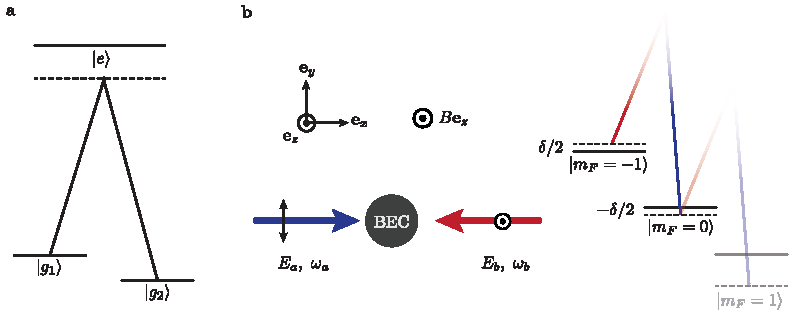
\includegraphics[]{Figures/Chapter3/Raman_coupling.pdf}
\caption[Raman coupling with two-photon transitions]{\note{TODO:write caption}}
\label{fig:Raman_coupling}
\end{center}
\end{figure*}

Consider two laser beams counter propagating along $\ex$ and with polarizations along $\ey$ and $\ez$ as is shown in Figure~\ref{fig:Raman_coupling}b. The electric field from the Raman beams is given by
%
\begin{equation}
  \mathbf{E}(x,t) = E_a\cos(k_a x-\omega_at)\e_y + E_b\cos(k_b x+\omega_bt)\ez,
\end{equation} 
%
and consequently 
%
\begin{equation}
	\mathbf{E}^*\times\mathbf{E} = 2i E_a E_b\cos(2\kl x-\Delta\omega t)\ex,
\end{equation}
%
where $\Delta\omega=\omega_a-\omega_b$. The geometry and wavelength of the Raman fields determine the natural units of the system: the single photon recoil momentum $k_{\mathrm{L}}=2\pi/\lambda_{\mathrm{R}}$ and its associated recoil energy $E_{\mathrm{L}}=\hbar^2k_{\mathrm{L}}^2/2m$, as well as the direction of the recoil momentum $\mathbf{k}_{\mathrm{L}}=k_{\mathrm{L}}\ex$. For most experiments we tune to the magic wavelength $\lambda_{\mathrm{R}}=790.032\,\nm$, so that the scalar light shift is zero and the scattering rate is minimized. We occasionally tuned away from this wavelength, for example when we were starving for laser power and wanted to increase our Raman coupling strength; Figure~\ref{fig:Raman_vs_lambda} shows the dependence of the Raman coupling strength and the lifetime on wavelength. 

\begin{figure*}[htb]
\begin{center}
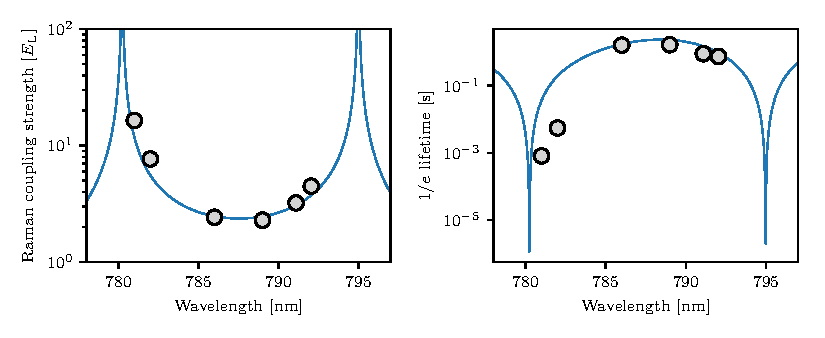
\includegraphics[]{Figures/Chapter3/Raman_vs_lambda.pdf}
\caption[Raman coupling strength and scattering rate as a function of wavelength]{Raman coupling strength and $1/e$ lifetime as a function of wavelength for a pair of Raman beams with waist $w_0\sim \unit[150]{\mu m}$ and powers of $~\unit[50, 10]{\mu W}$.}
\label{fig:Raman_vs_lambda}
\end{center}
\end{figure*}

The Raman Hamiltonian is given by
%
\begin{equation}
	\hat{H}_{R}=\Omega\cos(2\kl x-\Delta\omega t)\fx
\end{equation}
%
where $\Omega=\alpha^{(1)}g_F E_a E_b/g_J\propto \sqrt{I_a I_b}$ is the Raman coupling strength. In a frame rotating with angular frequency $\Delta\omega$ corresponding to applying the unitary transformation $\hat{U}(t)=\exp(-i\Delta\omega t\fz)$ and neglecting the fast terms rotating at frequency $2\Delta\omega$ (applying a RWA) the transformed Hamiltonian is
%
\begin{equation}
	\hat{U}^{\dagger}\hat{H}_R\hat{U} - i\hbar\hat{U}^{\dagger}\partial_t\hat{U}=\Delta\omega \fz+\frac{\Omega}{2}\cos(2\kl x)\fx-\frac{\Omega}{2}\sin(2\kl x)\fy,
	\label{eq:basic_Raman}
\end{equation}
%
which describes a helically precessing magnetic field with period $\lambda_{\rm R}/2$ which is illustrated in Figure~\ref{fig:B_eff}.

\begin{figure*}[htb]
\begin{center}
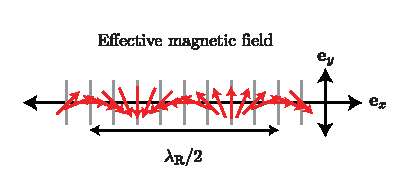
\includegraphics[]{Figures/Chapter3/B_eff.pdf}
\caption[Effective magnetic field from two cross polarized Raman laser beams]{The effective Raman Hamiltonian can be visualized as an interaction with an effective helically precessing magnetic field.}
\label{fig:B_eff}
\end{center}
\end{figure*}

\note{TODO: the two-level stuff maybe doesn't really make much sense anymore}


\subsection{Spin-orbit coupling}

The Raman Hamiltonian from Equation~\ref{eq:basic_Raman} can be massaged a bit more to make it look like a spin-orbit coupled\footnote{Not to be confused with the spin-orbit coupling giving rise to the fine and hyperfine structure mentioned earlier, perhaps a better name could be spin-momentum coupling} Hamiltonian that is familiar to condensed matter physicists. If we apply a spin-dependent momentum boost which is described by the unitary operator $\hat{U}(\kl)=\exp(i2\kl x \fz)$ the full Hamiltonian including the Raman coupling and the free 
%
\begin{equation}
 	\hat{H}_{\rm{SOC}} = \frac{\hbar^2}{2m}\left(\hat q_x-2\kl\fz\right)^2+\frac{\Omega}{2}\fx + \delta\fz + \hbar\epsilon\left(\mathds{1}-\frac{\fz^2}{\hbar^2}\right),
 \end{equation} 
%
where $\delta=E_-1-\Delta\omega$. We can go from an $F=1$ 3 system to an effective spin-$1/2$ system if we set $\Delta\omega=E_{-1}-E_0$ and consider a sizable quadratic Zeeman shift $\epsilon$, the $m_F=1$ state can be adiabatically eliminated. 
%
\begin{equation}
	\hat{H}_{SOC}=\frac{\hbar^2}{2m}(q_x-\kl\hat{\sigma}_y)^2+\frac{\hbar}{2}\Omega\hat{\sigma}_z + \frac{\hbar}{2}\delta\hat{\sigma}_y
\end{equation}
%
where $\sigma_{x,y,z}$ are the Pauli matrices. The Hamiltonian above corresponds to an equal superposition of Rashba-type~\cite{bychkov_oscillatory_1984} ($\propto \hat{\sigma}_xk_y-\hat{\sigma}_yk_x$) and Dresselhaus-type~\cite{dresselhaus_spin-orbit_1955} ($\propto -\sigma_xk_y-\sigma_y k_x$) SOC with an effective magnetic field $\propto\Omega$ in the $\ey-\ez$ plane~\cite{galitski_spin-orbit_2013,lin_spin-orbit-coupled_2011}. In Chapter~\ref{ch:Rashba} I discuss the Rashba term in more detail and introduce a way of engineering a system with only Rashba-type SOC using multiple internal levels and Raman transitions. 



\note{TODO: make plots of gamma, us and uv. Use data from atoms as an example?}

% In earlier sections we discussed the spin-orbit coupling interaction between spin and angular momentum that gives rise to the atomic level structure. In condensed matter systems, there is another kind of spin-orbit coupling that links the spin of the electrons with the linear or crystal momentum. In 2D materials, SOC can be represented as a sum of Rashba~\cite{bychkov_oscillatory_1984} and Dresselhaus~\cite{dresselhaus_spin-orbit_1955} SOC. 




\section{Floquet theory}



\section{Absorption imaging}
\subsection{Time of flight imaging}
Mention Stern Gerlach here
\subsection{Calibrating $I_{\rm{sat}}$}

%%%%%%%%%%%%%%%%%%%%%%%%%%%%%%%%%%%%%%%%%%%%%%%%%%%%%%%%%%%%%%%
%
%Graveyard
%
%%%%%%%%%%%%%%%%%%%%%%%%%%%%%%%%%%%%%%%%%%%%%%%%%%%%%%%%%%%%%

% The eigenstate of the perturbed Hamiltonian are linear combinations of the unperturbed eigenstates $\ket{n}$  
% %
% \begin{equation}
% 	\ket{\psi}=\sum_n a_n(t)e^{-iE_n t/\hbar}\ket{n},
% \end{equation}
% %
% using the time-dependent Schr\"odinger equation we can find equations for the coefficients $a_n(t)$
% %
% \begin{equation}
% 	i\hbar \partial_ta_n(t)=\sum_k\bra{n}\hat{H}_{\rm{dip}}\ket{k}a_k(t)e^{i\omega_{n,k}t}
% \end{equation}
% %
% where $\omega_{nk}=(E_n-E_k)/\hbar$. If we consider the perturbation being turned on at $t=0$ and if $\omega\neq\omega_{nk}$ the first order coefficient is
% %
% \begin{equation}
% 	a_n^{(1)}=-\frac{\bra{n}d_iE_0\ket{m}}{2\hbar}
% \end{equation}

% For $S$ electrons the hyperfine splitting can be described by the Hamiltonian $\hat H_{\rm{hfs}} = A_{\rm{hfs}}\mathbf{I}\cdot\mathbf{J}$\footnote{Notice how both the fine and hyperfine structure arise from a spin-orbit coupling interaction, we will discuss a very different type of spin-orbit coupling in future chapter.}. Figure~\ref{fig:fs_hfs}c shows the fine structure getting further split into states of total angular momentum $\mathbf{F}=\mathbf{J}+\mathbf{I}$. $\Rb87$ has a nuclear spin $I=3/2$ and therefore its ground state hyperfine configuration has $F=1$ and $F=2$. Here
% ~\cite{Steck} 

% Lets now consider the example of an atom in the presence of an oscillating electric field with amplitude $E_0$ and polarization $\epsilon$ $\mathbf{E}=E_0\cos(\omega t)\boldsymbol{\epsilon}$. We will use time-dependent perturbation theory to calculate the resulting energy shifts. 


% So far I have considered that the excited state has an infinitely long lifetime and does not decay. However, in reality the atom can spontaneously emit photons and decay. The lifetime of the excited state is given by $1/\Gamma_{e_j}$. The exponential decay of the excited state corresponds to adding a imaginary contribution to the energy $E_{e_j}\rightarrow E_{e_j}-i\hbar\Gamma_{e_j}/2$ which makes the polarizability a complex valued number. 

% The decay rate of a transition is related to the square of the dipole matrix element via Fermi's golden rule~\cite{Sakurai}

% \begin{equation}
% 	\Gamma_{J_gJ_e}=\frac{\omega_0^2}{3\pi\epsilon_0\hbar c^3}\frac{2J_g+1}{2J_e+1}\vert\langle g \| \mathbf{d}\|e\rangle\vert^2
% \end{equation}

% where $\vert\langle g \| \mathbf{d}\|e\rangle\vert^2$ is a reduced matrix element
% I will now look at the scalar polarizability term for Alkali atoms. For the case of far-detuned light such that the hyperfine $F$ levels are not well resolved the scalar polarizability can be calculated using the fine structure $J$ states. For an atom in an initial state $J$

% use scattering rate to find reduced matrix element write final expresion. skip the j, go back to generic notation
% %
% \begin{equation}
%  	\alpha^{(0)}\approx\sum_{J'}\frac{\vert\langle J \| \mathbf{d}\|J'\rangle \vert^2}{3\hbar}\left(\frac{1}{\omega+\omega_{JJ'}}-\frac{1}{\omega-\omega_{JJ'}}\right)
%  \end{equation} 
% If we consider Alkali atoms in the ground state hyperfine manifold in the presence of far detuned light such that the hyperfine levels are not well resolved we need to calculate the matrix elements using the $J$ states


% the scalar polarizability takes the form 
% The matrix element in Equation~\ref{eq:scalar_pol} can be expressed using the Wigner-Eckart theorem~\cite{Sakurai} in terms of the Clebsch-Gordan coefficients and the reduced matrix elements. 
%Here I will only consider the case of oscillating electric fields $\mathbf{E}=E_0\cos(\omega t)\boldsymbol{\epsilon}$ (i.e. plane waves of electromagnetic radiation) which are relevant to our experiments. 

% write tensor polarizability, write it into irreducible components. Mention that tensor component is very small and ignored. 

% Scalar polarizability: real part is light shift, complex part is scattering. Apply rwa and get the classic expressions for trapping potential and scattering. Make plot of polarizabily for RB87 Sub subsection: dipole traps

% Tensor polarizability



% Can break interaction into scalar, vector and tensor part. Interaction can also be resonant or off-resonant.

% \note{Why do you only get second order perturbation theory effects? I think it has something to do with unperturbed atomic states being eigenstates of the parity operator}

% We use light tuned to the magic wavelength $\lambda_{\mathrm{R}}=790.032\,\nm$ so that the scalar light shift vanishes (Section~\ref{sec:scalar_light_shift}). Because the light is considerably detuned from the D1 and D2 lines we do not take into account coupling into any of the excited states\footnote{Some atoms are inevitably excited of course, leading to heating from spontaneous emission (Equation~\ref{eq:scattering})}

% \note{Something about what we use this transitions for and how we usually ignore all other levels. (???)}

% \note{TODO: what about matrix elements between -1 and +1?. Move to intro chapter}


%%
%% This is file `supertabular.sty',
%% generated with the docstrip utility.
%%
%% The original source files were:
%%
%% supertabular.dtx  (with options: `package')
%% Copyright (C) 1989-2004 Johannes Braams. All rights reserved.
%% 
%% This file was generated from file(s) of the supertabular package.
%% -----------------------------------------------------------------
%% 
%% It may be distributed and/or modified under the
%% conditions of the LaTeX Project Public License, either version 1.3
%% of this license or (at your option) any later version.
%% The latest version of this license is in
%%   http://www.latex-project.org/lppl.txt
%% and version 1.3 or later is part of all distributions of LaTeX
%% version 2003/12/01 or later.
%% 
%% This work has the LPPL maintenance status "maintained".
%% 
%% The Current Maintainer of this work is Johannes Braams.
%% 
%% This file may only be distributed together with a copy of the
%% supertabular package. You may however distribute the supertabular package
%% without such generated files.
%% 
%% The list of all files belonging to the supertabular package is
%% given in the file `manifest.txt.
%% 
%% The list of derived (unpacked) files belonging to the distribution
%% and covered by LPPL is defined by the unpacking scripts (with
%% extension .ins) which are part of the distribution.
%% Sourcefile `supertabular.dtx'.
%%
%% Copyright (C) 1988 by Theo Jurriens
%% Copyright (C) 1990-2004 by Johannes Braams texniek at braams.cistron.nl
%%                            Kersengaarde 33
%%                            2723 BP Zoetermeer NL
%%                       all rights reserved.
%%
%%
\NeedsTeXFormat{LaTeX2e}
\ProvidesPackage{supertabular}
              [2004/02/20 v4.1e the supertabular environment]
\newcount\c@tracingst
\DeclareOption{errorshow}{\c@tracingst\z@}
\DeclareOption{pageshow}{\c@tracingst\tw@}
\DeclareOption{debugshow}{\c@tracingst5\relax}
\ProcessOptions
\newif\if@topcaption \@topcaptiontrue
\def\topcaption{\@topcaptiontrue\tablecaption}
\def\bottomcaption{\@topcaptionfalse\tablecaption}
\long\def\tablecaption{%
  \refstepcounter{table}\@dblarg{\@xtablecaption}}
\long\def\@xtablecaption[#1]#2{%
  \long\gdef\@process@tablecaption{\ST@caption{table}[#1]{#2}}}
\global\let\@process@tablecaption\relax
\newif\ifST@star
\newif\ifST@mp
\newdimen\ST@wd
\newskip\ST@rightskip
\newskip\ST@leftskip
\newskip\ST@parfillskip
\long\def\ST@caption#1[#2]#3{\par%
  \addcontentsline{\csname ext@#1\endcsname}{#1}%
                  {\protect\numberline{%
                      \csname the#1\endcsname}{\ignorespaces #2}}
  \begingroup
    \@parboxrestore
    \normalsize
    \if@topcaption \vskip -10\p@ \fi
    \@makecaption{\csname fnum@#1\endcsname}{\ignorespaces #3}\par
    \if@topcaption \vskip 10\p@ \fi
  \endgroup}
\newcommand\tablehead[1]{%
  \gdef\@tablehead{%
  \noalign{%
      \global\let\@savcr=\\
      \global\let\\=\org@tabularcr}%
    #1%
    \noalign{\global\let\\=\@savcr}}}
\tablehead{}
\newcommand\tablefirsthead[1]{\gdef\@table@first@head{#1}}
\newcommand\tabletail[1]{%
  \gdef\@tabletail{%
    \noalign{%
      \global\let\@savcr=\\
      \global\let\\=\org@tabularcr}%
    #1%
    \noalign{\global\let\\=\@savcr}}}
\tabletail{}
\newcommand\tablelasttail[1]{\gdef\@table@last@tail{#1}}
\newcommand\sttraceon{\c@tracingst5\relax}
\newcommand\sttraceoff{\c@tracingst\z@}
\newcommand\ST@trace[2]{%
  \ifnum\c@tracingst>#1\relax
    \GenericWarning
      {(supertabular)\@spaces\@spaces}
      {Package supertabular: #2}%
  \fi
  }
\newdimen\ST@pageleft
\newcommand*\shrinkheight[1]{%
  \noalign{\global\advance\ST@pageleft-#1\relax}}
\newcommand*\setSTheight[1]{%
  \noalign{\global\ST@pageleft=#1\relax}}
\newdimen\ST@headht
\newdimen\ST@tailht
\newdimen\ST@pagesofar
\newdimen\ST@pboxht
\newdimen\ST@lineht
\newdimen\ST@stretchht
\newdimen\ST@prevht
\newdimen\ST@toadd
\newdimen\ST@dimen
\newbox\ST@pbox
\def\ST@tabularcr{%
  {\ifnum0=`}\fi
  \@ifstar{\ST@xtabularcr}{\ST@xtabularcr}}
\def\ST@xtabularcr{%
  \@ifnextchar[%]
    {\ST@argtabularcr}%
    {\ifnum0=`{\fi}\cr\ST@cr}}
\def\ST@argtabularcr[#1]{%
  \ifnum0=`{\fi}%
  \ifdim #1>\z@
    \unskip\ST@xargarraycr{#1}
  \else
    \ST@yargarraycr{#1}%
  \fi}
\def\ST@xargarraycr#1{%
  \@tempdima #1\advance\@tempdima \dp \@arstrutbox
  \vrule \@height\z@ \@depth\@tempdima \@width\z@ \cr
  \noalign{\global\ST@toadd=#1}\ST@cr}
\def\ST@yargarraycr#1{%
  \cr\noalign{\vskip #1\global\ST@toadd=#1}\ST@cr}
\def\ST@startpbox#1{%
  \setbox\ST@pbox\vtop\bgroup\hsize#1\@arrayparboxrestore}
\def\ST@astartpbox#1{%
  \bgroup\hsize#1%
  \setbox\ST@pbox\vtop\bgroup\hsize#1\@arrayparboxrestore}
\def\ST@endpbox{%
  \@finalstrut\@arstrutbox\par\egroup
  \ST@dimen=\ht\ST@pbox
  \advance\ST@dimen by \dp\ST@pbox
  \ifnum\ST@pboxht<\ST@dimen
    \global\ST@pboxht=\ST@dimen
  \fi
  \ST@dimen=\z@
  \box\ST@pbox\hfil}
\def\ST@aendpbox{%
  \@finalstrut\@arstrutbox\par\egroup
  \ST@dimen=\ht\ST@pbox
  \advance\ST@dimen by \dp\ST@pbox
  \ifnum\ST@pboxht<\ST@dimen
    \global\ST@pboxht=\ST@dimen
  \fi
  \ST@dimen=\z@
  \unvbox\ST@pbox\egroup\hfil}
\def\estimate@lineht{%
  \ST@lineht=\arraystretch \baslineskp
  \global\advance\ST@lineht by 1\p@
  \ST@stretchht\ST@lineht\advance\ST@stretchht-\baslineskp
  \ifdim\ST@stretchht<\z@\ST@stretchht\z@\fi
  \ST@trace\tw@{Average line height: \the\ST@lineht}%
  \ST@trace\tw@{Stretched line height: \the\ST@stretchht}%
  }
\def\@calfirstpageht{%
  \ST@trace\tw@{Calculating height of tabular on first page}%
  \global\ST@pagesofar\pagetotal
  \global\ST@pageleft\@colroom
  \ST@trace\tw@{Height of text = \the\pagetotal; \MessageBreak
                Height of page = \the\ST@pageleft}%
  \if@twocolumn
    \ST@trace\tw@{two column mode}%
    \if@firstcolumn
     \ST@trace\tw@{First column}%
      \ifnum\ST@pagesofar > \ST@pageleft
        \global\ST@pageleft=2\ST@pageleft
        \ifnum\ST@pagesofar > \ST@pageleft
          \newpage\@calnextpageht
          \ST@trace\tw@{starting new page}%
        \else
          \ST@trace\tw@{Second column}%
          \global\advance\ST@pageleft -\ST@pagesofar
          \global\advance\ST@pageleft -\@colroom
        \fi
      \else
        \global\advance\ST@pageleft by -\ST@pagesofar
        \global\ST@pagesofar\z@
      \fi
    \else
      \ST@trace\tw@{Second column}
      \ifnum\ST@pagesofar > \ST@pageleft
        \ST@trace\tw@{starting new page}%
        \newpage\@calnextpageht
      \else
        \global\advance\ST@pageleft by -\ST@pagesofar
        \global\ST@pagesofar\z@
      \fi
    \fi
  \else
    \ST@trace\tw@{one column mode}%
    \ifnum\ST@pagesofar > \ST@pageleft
      \ST@trace\tw@{starting new page}%
      \newpage\@calnextpageht
    \else
      \global\advance\ST@pageleft by -\ST@pagesofar
      \global\ST@pagesofar\z@
    \fi
  \fi
  \ST@trace\tw@{Available height: \the\ST@pageleft}%
  \ifx\@@tablehead\@empty
    \ST@headht=\z@
  \else
    \setbox\@tempboxa=\vbox{\@arrayparboxrestore
      \ST@restore
      \expandafter\tabular\expandafter{\ST@tableformat}%
      \@@tablehead\endtabular}%
    \ST@headht=\ht\@tempboxa\advance\ST@headht\dp\@tempboxa
  \fi
  \ST@trace\tw@{Height of head: \the\ST@headht}%
  \ifx\@tabletail\@empty
    \ST@tailht=\z@
  \else
    \setbox\@tempboxa=\vbox{\@arrayparboxrestore
      \ST@restore
      \expandafter\tabular\expandafter{\ST@tableformat}
        \@tabletail\endtabular}
    \ST@tailht=\ht\@tempboxa\advance\ST@tailht\dp\@tempboxa
  \fi
  \advance\ST@tailht by \ST@lineht
  \ST@trace\tw@{Height of tail: \the\ST@tailht}%
  \ST@trace\tw@{Maximum height of tabular: \the\ST@pageleft}%
  \@tempdima\ST@headht
  \advance\@tempdima\ST@lineht
  \advance\@tempdima\ST@tailht
  \ST@trace\tw@{Minimum height of tabular: \the\@tempdima}%
  \ifnum\@tempdima>\ST@pageleft
    \ST@trace\tw@{starting new page}%
    \newpage\@calnextpageht
  \fi
}
\def\@calnextpageht{%
  \ST@trace\tw@{Calculating height of tabular on next page}%
  \global\ST@pageleft\@colroom
  \global\ST@pagesofar=\z@
  \ST@trace\tw@{Maximum height of tabular: \the\ST@pageleft}%
  }
\def\x@supertabular{%
  \let\org@tabular\tabular
  \let\tabular\inner@tabular
  \expandafter\let
    \csname org@tabular*\expandafter\endcsname
    \csname tabular*\endcsname
  \expandafter\let\csname tabular*\expandafter\endcsname
    \csname inner@tabular*\endcsname
  \if@topcaption \@process@tablecaption \fi
  \global\let\@oldcr=\\
  \def\baslineskp{\baselineskip}%
  \ifx\undefined\@classix
    \let\org@tabularcr\@tabularcr
    \let\@tabularcr\ST@tabularcr
    \let\org@startpbox=\@startpbox
    \let\org@endpbox=\@endpbox
    \let\@@startpbox=\ST@startpbox
    \let\@@endpbox=\ST@endpbox
  \else
    \let\org@tabularcr\@arraycr
    \let\@arraycr\ST@tabularcr
    \let\org@startpbox=\@startpbox
    \let\org@endpbox=\@endpbox
    \let\@startpbox=\ST@astartpbox
    \let\@endpbox=\ST@aendpbox
  \fi
  \ifx\@table@first@head\undefined
    \let\@@tablehead=\@tablehead
  \else
    \let\@@tablehead=\@table@first@head
  \fi
  \let\ST@skippage\ST@skipfirstpart
  \estimate@lineht
  \@calfirstpageht
  \noindent
  }
\def\supertabular{%
  \@ifnextchar[{\@supertabular}%]
               {\@supertabular[]}}
\def\@supertabular[#1]#2{%
  \def\ST@tableformat{#2}%
  \ST@trace\tw@{Starting a new supertabular}%
  \global\ST@starfalse
  \global\ST@mpfalse
  \x@supertabular
  \expandafter\org@tabular\expandafter{\ST@tableformat}%
  \@@tablehead}
\@namedef{supertabular*}#1{%
  \@ifnextchar[{\@nameuse{@supertabular*}{#1}}%
               {\@nameuse{@supertabular*}{#1}[]}%]
  }
\@namedef{@supertabular*}#1[#2]#3{%
  \ST@trace\tw@{Starting a new supertabular*}%
  \def\ST@tableformat{#3}%
  \ST@wd=#1\relax
  \global\ST@startrue
  \global\ST@mpfalse
  \x@supertabular
  \expandafter\csname org@tabular*\expandafter\endcsname
  \expandafter{\expandafter\ST@wd\expandafter}%
  \expandafter{\ST@tableformat}%
  \@@tablehead}%
\def\mpsupertabular{%
  \@ifnextchar[{\@mpsupertabular}%]
               {\@mpsupertabular[]}}
\def\@mpsupertabular[#1]#2{%
  \def\ST@tableformat{#2}%
  \ST@trace\tw@{Starting a new mpsupertabular}%
  \global\ST@starfalse
  \global\ST@mptrue
  \ST@rightskip \rightskip
  \ST@leftskip \leftskip
  \ST@parfillskip \parfillskip
  \x@supertabular
  \minipage{\columnwidth}%
  \parfillskip\ST@parfillskip
  \rightskip \ST@rightskip
  \leftskip \ST@leftskip
  \noindent\expandafter\org@tabular\expandafter{\ST@tableformat}%
  \@@tablehead}
\@namedef{mpsupertabular*}#1{%
  \@ifnextchar[{\@nameuse{@mpsupertabular*}{#1}}%
               {\@nameuse{@mpsupertabular*}{#1}[]}%]
  }
\@namedef{@mpsupertabular*}#1[#2]#3{%
  \ST@trace\tw@{Starting a new mpsupertabular*}%
  \def\ST@tableformat{#3}%
  \ST@wd=#1\relax
  \global\ST@startrue
  \global\ST@mptrue
  \ST@rightskip \rightskip
  \ST@leftskip \leftskip
  \ST@parfillskip \parfillskip
  \x@supertabular
  \minipage{\columnwidth}%
  \parfillskip\ST@parfillskip
  \rightskip \ST@rightskip
  \leftskip \ST@leftskip
  \noindent\expandafter\csname org@tabular*\expandafter\endcsname
  \expandafter{\expandafter\ST@wd\expandafter}%
  \expandafter{\ST@tableformat}%
  \@@tablehead}%
\def\endsupertabular{%
  \ifx\@table@last@tail\undefined
    \@tabletail
  \else
    \@table@last@tail
  \fi
  \csname endtabular\ifST@star*\fi\endcsname
  \ST@restore
  \if@topcaption
  \else
    \@process@tablecaption
    \@topcaptiontrue
  \fi
  \global\let\\\@oldcr
  \global\let\@process@tablecaption\relax
  \ST@trace\tw@{Ended a supertabular\ifST@star*\fi}%
  }
\expandafter\let\csname endsupertabular*\endcsname\endsupertabular
\def\endmpsupertabular{%
  \ifx\@table@last@tail\undefined
    \@tabletail
  \else
    \@table@last@tail
  \fi
  \csname endtabular\ifST@star*\fi\endcsname
  \endminipage
  \ST@restore
  \if@topcaption
  \else
    \@process@tablecaption
    \@topcaptiontrue
  \fi
  \global\let\\\@oldcr
  \global\let\@process@tablecaption\relax
  \ST@trace\tw@{Ended a mpsupertabular\ifST@star*\fi}%
  }
\expandafter\let\csname endmpsupertabular*\endcsname\endmpsupertabular
\def\ST@restore{%
  \ifx\undefined\@classix
    \let\@tabularcr\org@tabularcr
  \else
    \let\@arraycr\org@tabularcr
  \fi
  \let\@startpbox\org@startpbox
  \let\@endpbox\org@endpbox
  }
\def\inner@tabular{%
  \ST@restore
  \let\\\@oldcr
  \noindent
  \org@tabular}
\@namedef{inner@tabular*}{%
  \ST@restore
  \let\\\@oldcr
  \noindent
  \csname org@tabular*\endcsname}
\def\ST@cr{%
  \noalign{%
    \ifnum\ST@pboxht<\ST@lineht
      \global\advance\ST@pageleft -\ST@lineht
      \global\ST@prevht\ST@lineht
    \else
     \ST@trace\thr@@{Added par box with height \the\ST@pboxht}%
      \global\advance\ST@pageleft -\ST@pboxht
      \global\advance\ST@pageleft -0.1\ST@pboxht
      \global\advance\ST@pageleft -\ST@stretchht
      \global\ST@prevht\ST@pboxht
      \global\ST@pboxht\z@
    \fi
    \global\advance\ST@pageleft -\ST@toadd
    \global\ST@toadd=\z@
    \ST@trace\thr@@{Space left for tabular: \the\ST@pageleft}%
  }
  \noalign{\global\let\ST@next\@empty}%
  \ifnum\ST@pageleft<\z@
    \ST@skippage
  \else
    \noalign{\global\@tempdima\ST@tailht
      \global\advance\@tempdima\ST@prevht
    \ifST@mp
      \ifvoid\@mpfootins\else
        \global\advance\@tempdima\ht\@mpfootins
        \global\advance\@tempdima 3pt
      \fi
    \fi}
    \ifnum\ST@pageleft<\@tempdima
      \ST@newpage
    \fi
  \fi
  \ST@next}
\def\ST@skipfirstpart{%
  \noalign{%
    \ST@trace\tw@{Tabular too high, moving to next page}%
    \global\advance\ST@pageleft\pagetotal
    \global\ST@pagesofar\z@
    \newpage
    \global\let\ST@skippage\ST@newpage
    }}
\def\ST@newpage{%
  \noalign{\ST@trace\tw@{Starting new page, writing tail}}%
  \@tabletail
  \ifST@star
    \csname endtabular*\endcsname
  \else
    \endtabular
  \fi
  \ifST@mp
    \endminipage
  \fi
  \global\let\ST@skippage\ST@newpage
  \newpage\@calnextpageht
  \let\ST@next\@tablehead
  \ST@trace\tw@{writing head}%
  \ifST@mp
    \noindent\minipage{\columnwidth}%
    \parfillskip\ST@parfillskip
    \rightskip \ST@rightskip
    \leftskip \ST@leftskip
  \fi
  \noindent
  \ifST@star
    \expandafter\csname org@tabular*\expandafter\endcsname
    \expandafter{\expandafter\ST@wd\expandafter}%
    \expandafter{\ST@tableformat}%
  \else
    \expandafter\org@tabular\expandafter{\ST@tableformat}%
  \fi}
\endinput
%%
%% End of file `supertabular.sty'.

\titleformat{\chapter}
      {\normalfont\large}{Appendix \thechapter:}{1em}{}
%Appendix -- January 2015
\appendix
\renewcommand{\thechapter}{A}
\renewcommand{\chaptername}{Appendix}

\chapter{Experiments with partial transfer absorption imaging}


%Appendix -- January 2015
\appendix
\renewcommand{\thechapter}{B}
\renewcommand{\chaptername}{Appendix}

\chapter{New apparatus}
\label{app:new_apparatus}

As mentioned in the main text, the construction of a new apparatus for producing BECs of $\Rb87$ and $^{39}$K is underway. The design of the apparatus is intended to be a bug fix version of the RbChip~\cite{AbyThesis} lab at NIST. The new apparatus does not have a Zeeman slower and instead will use magnetic transport coils to move atoms from a MOT cell to the main science cell. 

This Appendix describes some aspects of the design and construction of the new apparatus where I was involved. Disclaimer: none of this things have been tested yet so we don't know yet if it will all work horribly. I have listed all relevant part numbers in case replacements are needed. 

\section{Water cooling}

The lack of a Zeeman slower in the apparatus greatly simplifies the water cooling system compared to that of RbLi. Since we don't anticipate to have any coils with high flow impedance we expect that the pressure from a recirculating chiller will be enough to provide water cooling to the transistor banks and the magnetic transport coils. 

Our choice of chiller was the \noted{TF1LN400-LN} $\unit[1.4]{kW}$ recirculating chiller from \noted{Thermo Fisher Scientific}. The water is filtered both at the output and the return with a high-impedance filter with a cellulose cartridge (filter: Mcmaster \noted{4422K3}, cartridge: McMater \noted{7191K11}). A breakout manifold divides the chilled water into 5 different lines, each one with a flow meter (\noted{Proteus Industries 0101C110}) that can be used to interlock the current of water cooled applications to the flow of water. Based on previous experiences with plumbing (see Appendix~\ref{app:RbLi}) I highly encourage replacing the filters at least once a year and to use a solution of $10\%$ corrosion inhibitor (e.g. OptiShield Plus) and distilled water as a coolant. 

\begin{figure*}[htb]
\begin{center}
\includegraphics[]{Figures/AppendixB/plumbing.pdf}
\caption[Water cooling]{Water cooling}
\label{fig:plumbing}
\end{center}
\end{figure*}

\section{Electrical installation}
We have two \noted{Agilent 6690A} ($\unit[440]{A}$ at $\unit[15]{V}$ max. current) to provide all the necessary currents. The power supplies are located in the service corridor and are connected to three copper bars corresponding to $\unit[\pm 15]{V}$ and ground using welding cable (McMaster \noted{7818A17}) that is laid on cable trays (McMaster \noted{30065T11} e.g.). The positive and negative terminals of the power supples have two cables attached to them and they are all arranged in the pattern shown in Figure~\ref{fig:welding_cables} so that the magnetic field produced by them is closer to a magnetic quadrupole which decays faster than the field of a magnetic dipole. This means we disturb our lab as well as neighboring labs less whenever we are running high currents. We are not planing to use commercial bipolar power supplies in this lab (see Appendix~\ref{app:RbLi}) and instead we will be using a MOSFET based homemade device that will draw current from the $\unit[\pm15]{V}$ rails. 

\begin{figure*}[htb]
\begin{center}
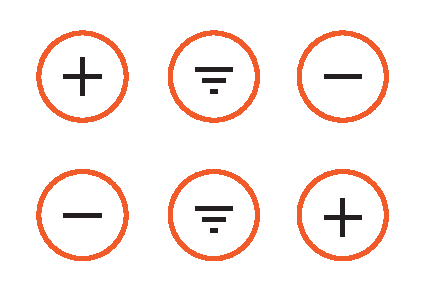
\includegraphics[]{Figures/AppendixB/welding_cables.pdf}
\caption{Configuration of the welding cables connecting the power supplies to equipment in the lab.}
\label{fig:welding_cables}
\end{center}
\end{figure*}
%
\begin{figure*}[htb]
\begin{center}
\includegraphics[]{Figures/AppendixB/electric.pdf}
\caption[Electrical installation]{A roller coaster ride, from the power supplies in the service corridor to three copper bars that distribute the power.}
\label{fig:electric}
\end{center}
\end{figure*}

\section{Coil winding}
All the coils in the apparatus including magnetic transport, bias and gradient cancellation have been wound using \noted{Laminax} ribbon wire from \noted{Bridgeport Magnetics}. We followed the the coil fabrication process described in~\cite{AbyThesis} which involves first winding a fixed number of turns around a prefabricated form with a particular geometry. The coils were then covered with a machinable epoxy (\noted{Stycast 1266}) to fill in any air gaps. A lesson we learned while doing this is that only room temperature epoxy should be mixed. We keep the epoxy in a fridge to extend its lifetime but if it is cold some tiny drops of water will condense in it as it is being mixed and it will not properly be cured. To minimize the air bubbles we placed the coils with epoxy on a vacuum bell and we pumped the air out using an electric vacuum pump (\noted{McMaster 4396K21}). After the epoxy has cured (overnight if it is left at room temperature or less if it is left at higher temperature) the coils are ready for lathing to remove all excess epoxy and kapton tape up to the surface of the copper. After some trial and error (and lots of frustration) we found that using a diamond tip cutter (\noted{McMaster 3316A32}) and spinning the lathe not faster than $\unit[150]{rpm}$ the best results. Using a cutter that is not sharp enough or cutting too aggressively close to the soft copper results in deformed rather. In the past when coils were fabricated at NIST a lathing form was used to mount the coils on the lathe. The machinist at UMD considered this was not safe enough so I instead mounted the coils using a 6 jaw chuck as shown in Figure~\ref{fig:coil_winding}a. than cut traces that merge into each other causing unwanted shorts. For anyone making coils in the future: it is sort of an art to get it right and screwing up many coils is part of learning the art. 

\begin{figure*}[htb]
\begin{center}
\includegraphics[]{Figures/AppendixB/coil_winding.pdf}
\caption[Lathing of magnetic transport coils]{{\bf a.} I used a six jaw chuck and a diamond cutter on the lathe to remove the excess epoxy and kapton on the coils. {\bf b.} Coils before (left) and after lathing (right). {\bf c.} A good labeling system is important to keep to ensure uniformity of coils. The `Wartortle' coil shown here has 64 turns. During fabrication we keep track of all the number of turns and resistance of all coils in a table.}
\label{fig:coil_winding}
\end{center}
\end{figure*}

\section{Rb source and `oven'}
The Rb source consists of a $1.33"$ CF flanged bellow (\noted{Kurt J. Lesker} \noted{MH-CF-A03}) with a Rb ampule . The bellow is housed in a cold `oven' which is designed to keep the source at a temperature $\approx \unit[1]{C}$ to keep the vapor pressure low. The oven is made of hollow aluminum cylinder with a slit on one side with tapped holes so that $1/4-20$ screws can be used to fix the oven to the source. The bottom of the oven attaches to the cold end of a TEC that provides the cooling. The hot side of the TEC is attached to a heat sink made of a hollow brass piece with tapped holes for $1/4"$ NPT pipes are used to provide water cooling. The left panel of Figure xxx shows CAD drawings of the oven both of this parts and the right panel shows the actual parts mounted on a test bench. The Rb source will be connected to the MOT glass cell; the plan is to use light induced atomic desorption (LIAD)\cite{anderson_loading_2001} to increase the Rb vapor pressure for MOT loading using non-thermal means. 

We tested the performance of a prototype without any vacuum systems attached to it. We applied a $\unit[2]{A}$ current to two TECs (\noted{Digikey 102-1664-ND}) sandwiched in between the heat sink and oven. The heat sink was water cooled using $\approx[18]{C}$ water. Figure~\ref{fig:rb_source}b shows the temperature of both the oven side (top) and the heat sink side (bottom) of the assembly. We did not use any insulation for this test to prevent condensation (see Figure~\ref{fig:rb_source}c right) which should be done once its installed on the apparatus.

Our initial hope was to control the temperature using a linear temperature controller designed at the JQI (the design is available at the \href{https://github.com/JQIamo/Linear-Temperature-Controller}{JQI GitHub}) interfaced to the lab computer andLabscript using a serial to ethernet adapter (\noted{WIZnet WIZ107SR}). Unfortunately this project is not completed to this date.  

\begin{figure*}[htb]
\begin{center}
\includegraphics[]{Figures/AppendixB/rb_source.pdf}
\caption[Rubidium oven assembly]{Rubidium oven assembly}
\label{fig:rb_source}
\end{center}
\end{figure*}

\section{Table enclosures}
The enclosures of the optical tables are made of $\noted{Alumalite}$ from \noted{Laminators Inc.} mounted on frames made out of aluminum extrusions from \noted{80/20} and sliding tracks (\noted{2220} and \noted{2210}). Alumalite is a sandwich of a corrugated corrugated polypropylen material in between two thin sheets of aluminum. We chose this material because it is strong and lightweight. Its laser safety properties remain to be tested but we anticipate it is better than the acrylic panels at the RbLi lab. %The initial frames were designed and built mostly by former graduate student Daniel Campbell and later finished and modified by former undergraduate student Eliot Fenton, current graduate student Junheng Tao and me.  

To the new and future members of the lab: I sincerely hope the things I designed and built don't cause you much pain!



\renewcommand{\baselinestretch}{1}
\small\normalsize
\begin{thebibliography}{99}
\setlength{\parskip}{1em}

\bibitem{Agrawal1} G.P. Agrawal, {\em Nonlinear Fiber Optics} (Academic
Press, San Diego, CA, 2001), Chap. 1.
\bibitem{Bloembergen} N. Bloembergen, {\em Nonlinear Optics} (Benjamin,
Reading, MA, 1977).
\bibitem{Shen} Y.R. Shen, {\em Principles of Nonlinear Optics} (Wiley, New
York, 1984).
\bibitem{Butcher} P.N. Butcher and D.N. Cotter, {\em The Elements of
Nonlinear Optics} (Cambridge University Press, Cambridge, UK, 1990).
\bibitem{Boyd} R.W. Boyd, {\em Nonlinear Optics} (Academic Press, San Diego,
CA, 1992).
\bibitem{Newell} A.C. Newell and J.V. Moloney {\em Nonlinear Optics (Advanced Topics in the Interdisciplinary Mathematical Sciences)} (Westview Press, Boulder, CO, April 1992). 
\bibitem{Marcuse} D. Marcuse,{\em Light Transmission Optics} (Van Nostrand
Reinhold, New York, 1982), Chaps. 8 and 12.
\bibitem{Agrawal2} G.P. Agrawal, {\em Nonlinear Fiber Optics} (Academic
Press, San Diego, CA, 2001), Chap. 2.
\bibitem{Diament} P. Diament, {\em Wave Transmission and Fiber Optics}
(Macmillan, New York, 1990).
\bibitem{Zakharov} V.E. Zakharov and A.Shabat, Sov. Phys. JETP 
\textbf{34}, 62 (1972)
\bibitem{Hardin} R.H. Hardin and F.D. Tappert, SIAM
Rev. Chronicle \textbf{15}, 423 (1973).
\bibitem{Fisher} R.A.Fisher and
W.K. Bischel, Appl. Phys. Lett. \textbf{23}, 661 (1973); J. Appl. Phys
\textbf{46}, 4921 (1975).
\bibitem{Cooley} J.W. Cooley and J.W. Tukey,
Math. Comput. \textbf{19}, 297 (1965).
\bibitem{Trebino} R. Trebino, D.J. Kane, "Using phase retrieval to measure
the intensity and phase of ultrashort pulses: frequency resolved optical gating," J. Opt. Soc. Am. B \textbf{10}, 1101 (1993). 
\bibitem{Kanejqe} D.J. Kane, R. Trebino, "Characterization of Arbitrary Femtosecond Pulses Using Frequency-Resolved Optical Gating," IEEE J. Quant. Elect. \textbf{29}, 571 (1993). 
\bibitem{Kaneoptlett} D.J. Kane, R. Trebino, "Single-shot measurement of the intensity and phase of an arbitrary ultrashort pulse  by using frequency-resolved optical gating," Opt. Lett. \textbf{10}, 1101 (1993).
\bibitem{OShealett}P. O'Shea, M. Kimmel, X. Gu, R. Trebino, "Highly simplified device for ultrashort-pulse measurement," Opt. Lett. \textbf{26}, 932 (2001).
\bibitem{Agrawal3} G.P. Agrawal, {\em Nonlinear Fiber Optics} (Academic
Press, San Diego, CA, 2001), Chap. 3.
\bibitem{Agrawal4} G.P. Agrawal, {\em Nonlinear Fiber Optics} (Academic
Press, San Diego, CA, 2001), Chap. 4.
\bibitem{Agrawal10} G.P. Agrawal, {\em Nonlinear Fiber Optics} (Academic
Press, San Diego, CA, 2001), Chap. 10.
\bibitem{Agrawal7} G.P. Agrawal, {\em Nonlinear Fiber Optics} (Academic
Press, San Diego, CA, 2001), Chap. 7.
\bibitem{Agrawal6} G.P. Agrawal, {\em Nonlinear Fiber Optics} (Academic
Press, San Diego, CA, 2001), Chap. 6.
\bibitem{Stolen} R.H. Stolen, E.P. Ippen, and A.R. Tynes,
Appl. Phys. Lett. \textbf{20}, 62 (1972). 
\bibitem{Ippen} E.P. Ippen and R.H. Stolen, Appl. Phys. Lett. \textbf{21}, 
539 (1972). 
\bibitem{Smith} R.G. Smith, Appl. Opt. \textbf{11}, 2489 (1972).
\bibitem{Agrawal9} G.P. Agrawal, {\em Nonlinear Fiber Optics} (Academic
Press, San Diego, CA, 2001), Chap. 9.
\bibitem{Agrawal8} G.P. Agrawal, {\em Nonlinear Fiber Optics} (Academic
Press, San Diego, CA, 2001), Chap. 8.
\bibitem{hart1} D.L. Hart, Arthur F. Judy, Rajarshi Roy and James W. Beletic, Phys. Rev. E \textbf{57}, 4757 (1998); D.L. Hart, Arthur F. Judy, T.A.B. Kennedy, Rajarshi Roy and K. Stoev, Phys. Rev. A \textbf{50}, 1807 (1994).   
\bibitem{ito} K. Ito, {\em Lectures on Stochastic Processes} (Tata Institute of Fundamental Research, Bombay, 1960).
\bibitem{stratanovich} R.L. Stratanovich, {\em Topics in the Theory of Random Noise}, Vols I. and II. (Gordon \& Breach, New York, 1963).
\bibitem{risken} H. Risken, {\em The Fokker-Planck Equation} (Springer-Verlag, Berlin, 1989).
\bibitem{werner2} M.J. Werner and P.D. Drummond, J. Comput. Phys. \textbf{132}, 312 (1997).
\bibitem{drummond1} P.D. Drummond and I.K. Mortimer, J. Comput. Phys. \textbf{93}, 144 (1991).
\bibitem{carter3} S.J. Carter, Phys. Rev. A. \textbf{51}, 3274 (1995).
\bibitem{thompson1} J.R. Thompson and Rajarshi Roy, Phys. Rev. A \textbf{43}, 4987 (1991).
\bibitem{boxmuller} W.H. Press, S.A. Teukolsky, W.T. Vetterling and B.P. Flannery, {\em Numerical Recipes in Fortran: The Art of Scientific Computing} (Cambridge University Press, Cambridge, 1992).
\bibitem{headley} C. Headley, G.P. Agrawal, IEEE J. Quantum Electron. \textbf{QE-31}, 2058 (1995), C. Headley, G.P. Agrawal J. Opt. Soc. Am. B. \textbf{13}, 2170 (1995).
\bibitem{perlmutter1} S.H. Perlmutter, M.D. Levenson, R.M. Shelby and
M.B. Weisman, Phys. Rev. Lett. \textbf{61} 1388, 1988.
\bibitem{abdullaev} F. Kh. Abdullaev, J.H. Hensen, S. Bischoff and M.P. Sorensen, J. Opt. Soc. Am. B. \textbf{15}, 2424 (1998); F. Kh. Abdullaev, J.G. Caputo, and Nikos Flytzanis, Phys. Rev E. \textbf{50}, 1552 (1994).
\bibitem{glenn} William H. Glenn, IEEE J. Quantum Electron. \textbf{QE-25}, 1218 (1989).
\bibitem{Trebinobook} R. Trebino. {\em Frequency-Resolved Optical Gating: The Measurement of Ultrashort Laser Pulses} (Kluwer Academic 2002).
\bibitem{Agrawal} G.P. Agrawal {\em Nonlinear Fiber Optics} (Academic,
San Diego, 2001).
\bibitem{Dudley} J.M. Dudley, X. Gu, L. Xu, M. Kimmel, E. Zeek, P. O'Shea, R. Trebino, S. Coen, R.S. Windeler, "Cross-correlation frequency resolved optical gating analysis of broadband continuum generation in photonic crystal fiber: simulations and experiments," Opt. Express \textbf{10}, 1215 (2002).
\bibitem{Liu1} Q.D. Liu, J.T. Chen, Q.Z. Wang, P.P. Ho, and R.R. Alfano, "Single pulse degenerate-cross-phase modulation in a single-mode optical fiber," Opt. Lett. \textbf{20}, 542 (1995).
\bibitem{Sylvestre} T. Sylvestre, H. Maillotte, E. Lantz, and D. Gindre "Combined spectral effects of pulse walk-off and degenerate cross-phase modulation in birefringent fibers", Journal of Nonlinear Optical Physics and Materials 6, 313-320 (1997).
\bibitem{Liu2} Q.D. Liu, L. Shi, P.P. Ho, R.R. Alfano, R.J. Essiambre, and G.P. Agrawal, "Degenerate cross-phase modulation of femtosecond laser pulses in a birefringent single-mode fiber," IEEE Photon. Tech. Lett. \textbf{9}, 1107 (1997). 
\bibitem{Omenetto1} F.G. Omenetto, B.P. Luce, D. Yarotski and A.J. Taylor, "Observation of chirped soliton dynamics at l= 1.55 mm in a single-mode optical fiber with frequency-resolved optical gating," Opt. Lett. \textbf{24}, 1392 (1999).
% 1.55 micron regime - check for more recent papers by Omenetto use both web-sci and inspec
\bibitem{Omenetto2} F.G. Omenetto, Y. Chung, D. Yarotski, T. Shaefer, I. Gabitov and A.J. Taylor, "Phase analysis of nonlinear femtosecond pulse propagation and self-frequency shift in optical fibers," Opt. Commun. \textbf{208}, 191 (2002). 
\bibitem{Omenetto3} F.G. Omenetto, J.W. Nicholson, B.P. Luce, D. Yarotski, A.J. Taylor, "Shaping, propagation and characterization of ultrafast pulses in optical fibers," Appl. Phys. B \textbf{70}[Suppl.], S143 (2000).
\bibitem{Nishizawa1} N. Nishizawa and T. Goto, "Experimental analysis of ultrashort pulse propagation in optical fibers around zero-dispersion region using cross-correlation frequency resolved optical gating," Opt. Express \textbf{8}, 328 (2001).
\bibitem{Nishizawa2} N. Nishizawa and T. Goto, "Trapped pulse generation by femtosecond soliton pulse in birefringent optical fibers," Opt. Express \textbf{10}, 256 (2002).
\bibitem{Nishizawa3} N. Nishizawa and T. Goto, "Characteristics of pulse trapping by use of ultrashort soliton pulses in optical fibers across the zero-dispersion wavelength," Opt. Express \textbf{10}, 1151 (2002).
\bibitem{Nishizawa4} N. Nishizawa and T. Goto, "Ultrafast all optical switching by use of pulse trapping across zero-dispersion wavelength," Opt. Express \textbf{11}, 359 (2003).
% All of Nishizawa and Goto papers are related to 1.3 micron experiments and simulations.
\bibitem{Ogawa}, K. Ogawa, M.D. Pelusi, "Characterization of ultrashort optical pulses in a dispersion-managed fiber link using two-photon absorption frequency-resolved optical gating," Opt. Commun. \textbf{198}, 83-87 (2001).
\bibitem{Altes} R.A. Altes, "Detection, estimation, and classification
with spectrograms," J. Acoust. Soc. Am. \textbf{67}(4), 1232 (1980).
\bibitem{Christian} A. Christian Silva, "GRENOUILLE - Practical Issues," unpublished.
\bibitem{Mejia} J. Garduno-Mejia, A.H. Greenaway, and D.T. Reid, "Designer
femtosecond pulses using adaptive optics," Opt. Express \textbf{11}
2030 (2003).
\bibitem{OSheaexpress1} P. O'Shea, M. Kimmel, X. Gu, R. Trebino, "Increased-bandwidth in ultrashort-pulse measurement using an angle-dithered nonlinear-optical crystal," Opt. Express \textbf{7}, 342 (2000).
\bibitem{OSheaexpress2} P. O'Shea, M. Kimmel, R. Trebino, "Increased phase-matching bandwidth in simple ultrashort-laser-pulse measurements," J. Opt. B \textbf{4}, 44 (2002).
\bibitem{Akturk} S. Akturk, M. Kimmel, P. O'Shea, R. Trebino, "Measuring pulse-front tilt in ultrashort pulses using GRENOUILLE", Opt. Express \textbf{11}, 491 (2003).
\bibitem{Blow} K. J. Blow, D. Wood, "Theoretical Description of Transient Stimulated Raman Scattering in Optical Fibers," IEEE J. Quant. Elect. \textbf{25}, 2665 (1989).
\bibitem{Stolen2} R.H. Stolen, J.P. Gordon, W.J. Tomlinson,
J. Opt. Soc. Am. B \textbf{6}, 1159 (1989).
\bibitem{Mamyshev} P.V. Mamyshev and S.V. Chernikov, Sov. Lightwave
Commun. \textbf{2}, 97 (1992).
\bibitem{Headleythesis} C. Headley III, \em{Ultrafast Stimulated Raman
Scattering in Optical Fibers}, Ph.D. Thesis, University of Rochester,
NY (1995).
\end{thebibliography}

%When using Bibtex, delete the previous line and use the following
%three lines.  
%\newpage
%\bibliographystyle{unsrt} 
%\bibliography{Galactic,Dottie} %replace "Galactic,Dottie" with the
%                 file name(s) of your bib file(s)

\end{document}
